\documentclass[a4paper,12pt,oneside,openany,dvipdfmx,report]{jsbook}
\usepackage[dvipdfmx]{graphicx}
\usepackage{float}
%\usepackage{latexsym}
%\usepackage{txfonts}
\usepackage[fleqn]{amsmath}
\usepackage{amsthm}

\newtheorem{theorem}{Theorem}
\newtheorem{definition}[theorem]{Definition}
\newtheorem{lemma}[theorem]{Lemma}
\newtheorem{corollary}[theorem]{Corollary}


\pagestyle{plain}
\usepackage{here}
\usepackage[top=30truemm,bottom=30truemm,left=30truemm,right=30truemm]{geometry}
\title{\huge 時間と共に変化する多重集合に対するmin-hashの高速計算}
\author{2031136 三原 寛寿\\ 指導教員 古賀 久志 准教授\\  副指導教員  戸田 貴之}
\date{2022年1月28日}

\renewcommand{\baselinestretch}{1.2}
\makeatletter % プリアンブルで定義開始

% 表示文字列を"図"から"Figure"へ
%\renewcommand{\figurename}{Figure}

% 図番号を"<章番号>.<図番号>" へ
%t\renewcommand{\thefigure}{\thesection.\arabic{figure}}

% 章が進むごとに図番号をリセットする
%\@addtoreset{figure}{section}

\makeatother % プリアンブルで定義終了


\begin{document}
\maketitle
\large
\tableofcontents
\clearpage

\maketitle


\chapter{はじめに}
ストリームデータとは時間経過と共に継続的に次々と生成されるデータのことを言う.近年,IoTやSNSの発展に
伴いストリームデータが取り扱われる機会が増加している.例えば,IoTにおけるセンサからの観測データはストリーム
データである.また,特定ユーザのtwitterにおけるツイートやウェブぺージの閲覧履歴も時間と共に新データが
追加されるという点でストリームデータである.こうしてストリームデータの増加に連れて,ストリームデータを
対象とした類似検索も重要になっている.例えば,過去の異常パターンとの類似性に基づいた異常検知 \cite{microbiome} や,SNSの
コンテンツが似たユーザを見つけて類似ユーザの挙動からアイテムを推薦するユーザベースの情報推薦 \cite{POI} などは
ストリームデータを対象とした類似検索に帰着して解ける.後者の例では,ユーザ$u$のSNSへの投稿内容を時間経過に
伴ってデータが増えるストリームデータと見なし,ストリームデータを対象とした類似検索によって$u$と嗜好性が似た
類似ユーザを見つける.
最近のストリームデータを対象とした類似検索では,ストリームデータを生成されたデータの集合として表現し
集合間類似検索によって類似ストリームデータを探すアプローチが主流である.通常の集合間類似検索と比べると,
新たなデータの生成により集合の要素が動的に変化するため類似検索結果を更新する必要がある点が異なる.
2つの集合$A,B$に対する類似度$\mbox{sim}(A,B)$としてはJaccard係数がよく用いられるが,$A$や$B$が変化する度に
Jaccard係数を計算するオーバーヘッドは大きい.そこでMin-Hash \cite{Minhash}を用いて$A$と$B$のコンパクトなスケッチ
$ms_A,ms_B$を生成し,スケッチ間でJaccard係数を近似計算する手法がいろいろ提案されている.これらの手法はいずれ
も集合の変化に対するスケッチ更新を効率化するが,
\begin{itemize}
\item データ削除を取り扱えるか
\item 同種類の要素を複数持つ多重集合に対して拡張Jaccard係数の近似値を計算できるか
\end{itemize}
という2点で機能的に異なる.データ削除に関してはストリームデータ内では新しいデータほど最新の状況を反映して価値が高い
ところから, 古いデータを軽視するモデルが2種類存在する.
\begin{enumerate}
\item スライディングウィンドウモデル:データストリームの直近$w$個要素をスライディングウィンドウと定義し,
時刻が進むとウィンドウに到着データを追加し,ウィンドウ内の最古データを廃棄する.
\item 減衰モデル:データストリームを要素に重みが付与された重み付き集合として扱い,時間経過に伴って
古いデータの重みを減衰する.
\end{enumerate}
MaxLogHash \cite{Maxloghash}はMin-Hashを省メモリ化する$b$-bit Minhash\cite{b-bit}をデータ追加時に更新可能にした
がデータ削除を取り扱えない.Datarら\cite{Datar}はスライディングウィンドウモデルでデータ削除に対しても
ハッシュ値を更新できるアルゴリズムを考案した.さらにスケッチ更新のために保持しないといけないスライディング
ウィンドウ内の要素数が$O(\log W)$となることを証明した.$W$はスライディングウィンドウのサイズである.
しかし,Datarらの手法は多重集合を取り扱えない.Buryらは\cite{Bury}はデータ削除が任意の順序で発生しても
ハッシュ値を更新できる手法を構築したが,やはり多重集合は取り扱えない.Histosketch\cite{HistoSketch}は多重集合に関して
データ削除を取り扱える唯一の手法であるが,減衰モデルを想定している.したがって,スライディングウィンドウ
モデルで多重集合を取り扱える手法は存在しない.
そこで本研究では,スライディングウィンドウに対して多重集合を取り扱える手法を実現することを目的とし,
Datarらの手法を多重集合を取り扱えるように拡張する.多重集合の場合,スライディングウィンドウ内の同種類の要素数
に依って,同一要素に割り当てられるハッシュ値が変化するという難題があるが,本研究ではDatarらの手法をハッシュ値
の変化に対処できるように修正した.
%動的に変化する集合に対する効率的なMin-Hashスケッチの生成方法を
%研究対象とする.Xuらの近似解法ではクエリ集合が$Q_t$から$Q_{t+1}$に変化する度に,Min-Hashスケッチ$ms_{Q_{t+1}}$を完全
%に再計算する.しかし,$Q_t$と$Q_{t+1}$は多数の要素を共有するにもかかわらず,Min-Hashスケッチを完全に再計算するのは
%非効率である.$ms_{Q_{t+1}}$をMin-Hashスケッチ$ms_{Q_{t})}$を再利用して計算する手法が望まれるが,そのためには
%$Q_{t+1}$に対するMin-Hashのハッシュ値$h(Q_{t+1})$を,$Q_{t}$に対するハッシュ値$h(Q_{t})$を更新して計算出来なければ
%ならない.幸いそのような技術は既存であり,Datar[1]らがスライディングモデルに動的で変化する集合を対象
%としたハッシュ値更アルゴリズムを
%そこで本研究では,時間と共に変化する多重集合に対してMin-Hashのハッシュ値を更新できるように
%実験により,提案手法を用いて多重集合に対するMin-Hashスケッチを高速に計算できることを,集合間類似検索が高速に
%完了することから示した.集合間類似検索問題としては,データベースに$n$個のデータストリームのスライディングウィンドウにより
%定まる$n$個の動的に変化する集合$\{S^t_1,S^t_2,\cdots, S^t_n\}$が登録され,クエリ集合$Q$が静的な
%Continuous Similarity Search for Evolving Database問題[2]を取り扱った.
以下,本論文の構成を述べる.2章で提案手法の要素技術となる多重集合,集合間類似度,Min-Hashの概念を
説明する.3章では従来手法となるDatarらの動的に変化する集合を対象としたハッシュ値更アルゴリズムを紹介する.
4章で提案手法となる時間と共に変化する多重集合に対してMin-Hashのハッシュ値を更新アルゴリズムを提案する.
5章で4章のアルゴリズムを複数個の要素が出入りするウインドウに対応するように拡張したアルゴリズムを提案する.
6章で提案手法を人工データ,実データを用いて評価する.提案手法がハッシュ値を完全に再計算するベースライン手法
よりもMin-Hashスケッチを高速に更新できることを示す.%次にスケッチ更新のために保持しないといけないスライディングウィンドウ内の要素数が理論的に証明はできていないものの,実験的に$\log W$に比例することを示す.
7章でまとめと今後の課題を述べる.
%また,これらはユーザの嗜好性を表して
%いるため情報推薦に活用される.ここで,1データストリームを到着したデータの集りと捉えると,1データストリーム
%はユーザ嗜好性を表す動的に要素が追加される集合ということになる.従って,情報推薦は,動的に要素が追加%
%される集合に対する集合を対象とした
%さらに,
%このような背景の下、Xu[2]らは動的に変化する集合をクエリとして,静的な集合のデータベース$D$から
%毎時刻上位$K$個の類似集合を検索するContinuous Similarity Search for Evolving Queries問題を提唱とした.
%この問題設定では,クエリ集合$Q_t$をスライディングウィンドウで定義し,クエリ集合の変化に対応して検索結果を
%更新する必要がある.ここで$t$は時刻であり,クエリ集合が$t$によって変わることを表す.
%この問題は,$Q_t$とデータベース$D$の全集合間で,類似度(Jaccard係数)を毎時刻計算
%し,上位$k$個の集合を返すことで自明に厳密に解ける.しかし,この厳密解法では2つの集合$A$と$B$間で
%類似度$\mbox sim(A, B)$を計算するオーバーヘッドが大きい.そこで,Xuらは,Min-Hash[6]を用いて$A$と$B$のコンパクトなスケッチ
%(Min-Hashスケッチ)$ms_A,ms_B$[4]を生成し,スケッチ間でJaccard係数を近似計算する近似解法も提案している.

\chapter{準備}
\section{多重集合}
一般にオブジェクトの集まりを集合と呼ぶ.例えば\{a, b, c\}はアルファベットを要素とする集合である.一般的には要素群を表すアルファベット$\phi$に対して,その要素を0個以上含むものが集合となる.通常,集合は同じ種類の要素を1つしか含まない.集合を同じ種類の要素を複数持てるようにしたものを多重集合という.つまり,\{a, a, b, c, d, d, d\}というような集合である.


\section{Jaccard係数}
集合間で類似検索を行うには集合がどれだけ似ているのかを表す集合間類似度が定義されている必要がある.そのうちの1つとして,Jaccard係数がある.
Jaccard係数は,ある集合$A$と別の集合$B$について,以下の式\ref{eq:sim}で定義される.
\begin{equation}
\label{eq:sim}
\mathrm{sim}(A,B)=  \frac {|A \cap {B} |} {|A \cup {B}| }
\end{equation}

つまり,Jaccard係数は2つの集合に含まれている要素のうち共通要素が占める割合を表している.
例えば,$A=\{a,c,d,f,g\}$,$B=\{a,b,c,e,g,h,i\}$というような2つの集合が存在するとすると,${A \cup {B} }=\{a,b,c,d,e,f,g,h,i\}$,$ {A \cap {B} }=\{a,c,g\}$となり,類似度$sim(A,B)=0.375$となる.

そして,Jaccard係数を多重集合に拡張したものを拡張Jaccard係数と言う(式 \ref{eq:exjaccard}).
\begin{equation}
\label{eq:exjaccard}
\mathrm{sim}(A,B)=  \frac {\sum{\mathrm{min}\{a_i,b_i\}}} {\sum{\mathrm{max}\{a_i,b_i\}} }\\
\end{equation}

ここで,$a_i$は集合$A$が要素$i∈\phi$を含む個数である.

\section{Min-hash}
Min-hashとは,集合に対する確率的なハッシュ関数であり,Jaccard係数を用いた集合間類似検索を高速化するための技術である \cite{Minhash}.クエリとデータベースかの集合間でJaccard係数を計算することはJaccard係数計算のオーバーヘッドが大きい.その問題を改善し,Jaccard係数を高速に近似計算する方法として,Min-hashという計算方法が考えられた.Min-hashは計算されたハッシュ値が一致する確率はJaccard係数と一致するという性質を持ち,類似集合ほどハッシュ値が一致しやすいという良い性質を持つ(式\ref{eq:jaccard}).
%集合間類似検索とは,
%\begin{itemize}
%\item クエリ集合$Q$
%\item $n$の集合から構成されるデータベース$D=\{S_1,S_2,…,S_n\}$
%\end{itemize}
%が与えられて,データベース$D$から$Q$と類似した集合を見つける問題である.

%そして,Min-hashによって計算されたハッシュ値が一致する確率はJaccard係数と一致するという性質を持ち,類似集合ほどハッシュ値が一致しやすいという良い性質を持つ.(式\ref{eq:jaccard})
%Min-Hashはハッシュテーブルを用いてJaccard係数の計算回数を減らすことを目的としている.
\begin{equation}
$Pr[h(A)= h(B)]=sim(A,B)$
\label{eq:jaccard}
\end{equation}
$h$はハッシュ値であり,$A$,$B$は集合である.

次に,Min-hashによるハッシュ値の計算方法を紹介する.
$\phi=\{x_1,x_2,…,x_{|\phi|}\}$をアルファベット集合とする.ハッシュ関数は$\phi$の各アルファベットに対して,$\{1,2,…|\phi|\}$の中から被らないようにランダムな値を割り当てることで決定される(図2.1).1つのある集合の中のアルファベットを見て,その中の要素に対応する割り当て値の中から最小値を選ぶ.この最小値がMin-hashによるハッシュ値となる(式\ref{eq:datar}).
%\begin{figure}[H]
 % \centering
%  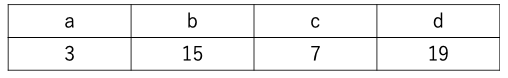
\includegraphics[width=9cm]{1wariate.png}
 % \caption{集合のハッシュ値表}
%\end{figure}


\begin{equation}
 \label{eq:datar}
h(A)=\min_{e \in \mbox{A}} \pi(e).
\end{equation}

さらに,Min-hashを用いたJaccard係数係数の近似計算を紹介する.
%元々,Min-Hashはハッシュテーブルを用いて,集合間類似検索を高速化することを目指して設計された一方で,
多数の要素を含む巨大な集合$A$のコンパクトな要約としてMin-Hashのハッシュ値を$k$個並べた\{$mh_1(A),mh_2(A),…,mh_k(A)$\}を使用するアプローチである.このMin-Hashのハッシュ値の集合を$A$のスケッチ \cite{Minhash}と呼ぶ.2つの集合$A$と$B$のスケッチ間で何個ハッシュ値が一致するかで $A $と$B$のハッシュ値を近似計算する.スケッチによって割り当てられる値はランダムに違うために,ハッシュ値もスケッチによって変わる.ハッシュ値が何個一致するかの確率はJaccard係数と一致するが,あくまで確率であるので,Min-Hashによるハッシュ値は近似値である.

\section{多重集合に対するMin-hash}
多重集合に対してMin-hashのハッシュ値を計算する手法を紹介する.文献では,大きく2つの方法が知られている.

(1)多重集合内の複数個のラベルに異なる値を割り当てる方法

(2)Consistent Weighted Sampling (CWS)  \cite{CWS} 

CWSは,Min-hashの出力の確率分布を模擬して,サンプリングすることでハッシュ値を計算する手法である.明示的に割り当て値を準備する必要がなく,多重集合が整数でなくても適用可能であるという利点がある.一方で確率の理論に精通していないと拡張が難しい手法でもある.(1)の同じラベルのアルファベットに異なる値を割り当てるやり方は多重集合の重みが整数であるという制約を受けるが,拡張は比較的容易な手法である.本論文では(1)の多重集合内の同一ラベルの要素に異なる値を割り当てる手法を使用する.

 
%多重集合において,集合の中に2つ以上同じアルファベットが存在することがある.多重集合に対するMin-Hashでは同一アルファベットに何個目かということに応じた異なる数値を割り当てる.

(1)のハッシュ値計算手法を例を用いて説明する.まず,図\ref{fig:2wariate}のように,アルファベット\{a,b,c,d\}に多重度が2である時の数値をランダムに割り当てる.
\begin{figure}[H]
  \centering
  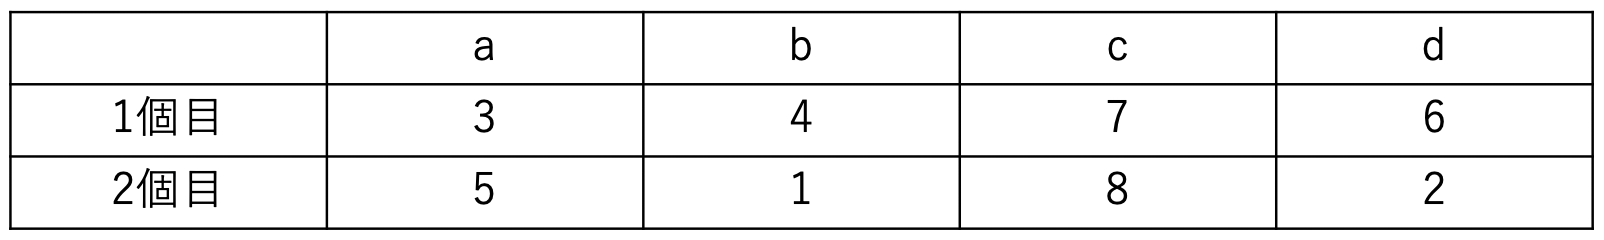
\includegraphics[width=15cm]{multi22.png}
  \caption{多重集合のハッシュ値表}
  \label{fig:2wariate}
\end{figure}

多重集合$A =\{a,b,b,c,c,d,d\}$とする.多重集合$A$に対して,図\ref{fig:2wariate}の割り当て表を用いて数値を割り当てる.そして,その中の最小値がMin-Hashによるハッシュ値となる(図\ref{fig:255}).

\begin{figure}[H]
  \centering
  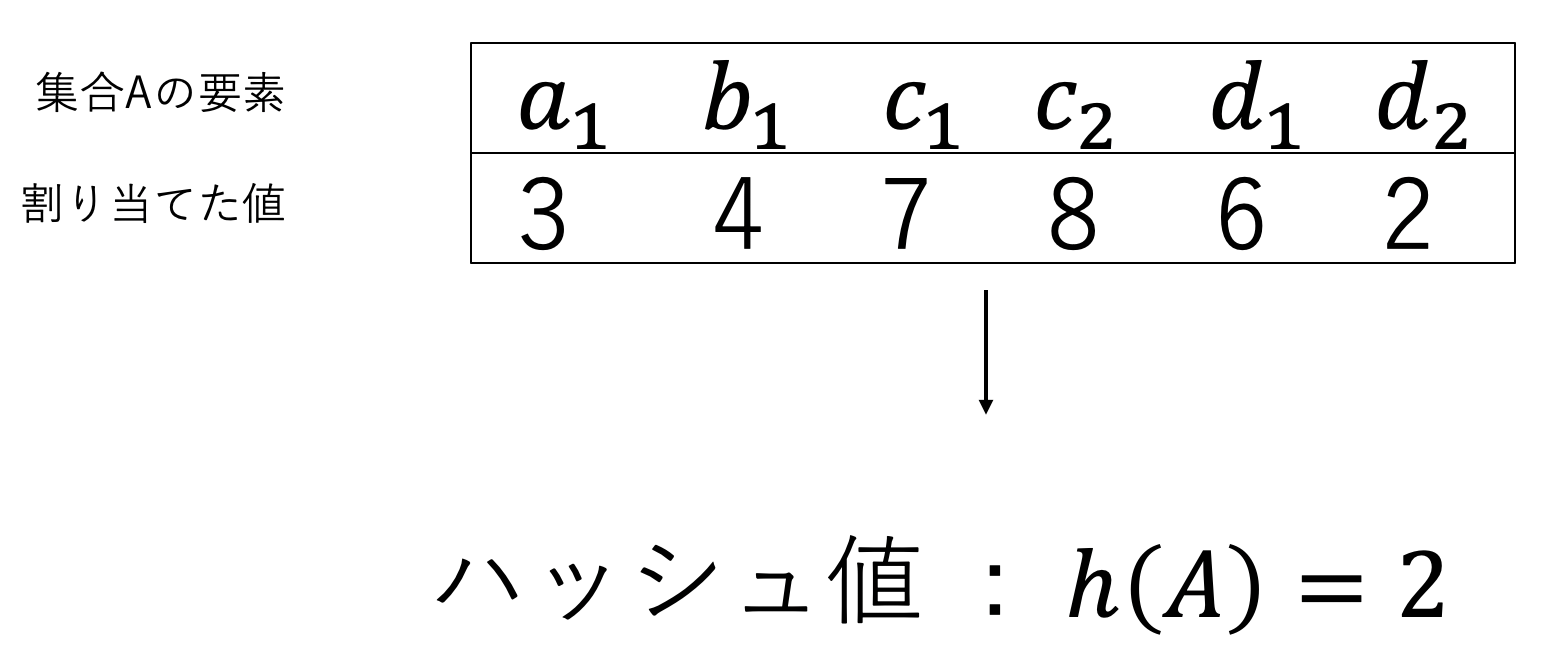
\includegraphics[width=15cm]{255.png}
  \caption{多重集合のハッシュ値計算}
  \label{fig:255}
\end{figure}


\chapter{Datarらのアルゴリズム}

本章では,Datarら \cite{Datar} によって提案されたデータストリームに対するハッシュ値更新アルゴリズムを
記述する.本論文での提案手法は,このアルゴリズムを基に多重集合へ拡張したものである.
データストリームとは,毎時刻要素$e$が到着するデータである.
Datarらの手法はデータストリームのスライディングウィンドウモデルに従って集合が変化することを仮定している.

\section{スライディングウインドウモデル}
時刻$t$における集合を$A_t=\{e_{t-w+1},e_{t-w+2},\cdots,e_t\}$とする.$w$はスライディングウインドウの幅であり,
$A_t$は$w$個の要素で構成される.また,$A_t$の要素は到着時間順に並んでいる.図\ref{fig:window}では,$w=4$の時
に3つの時刻$t$,$t+1$,$t+2$に対する集合$A_t,A_{t+1},A_{t+2}$を図示している.そして,時刻によってスライディングウインドウは変化していく.
例えば,図\ref{fig:window}のようにデータストリーム$\{a,f,h,e,k,q,o,g\}$となっていて,ウインドウサイズ$w=4$とすると,時刻$t$では,
$A_{t}=\{e_{t-3},e_{t-2},e_{t-1},e_t\}$であり,時刻$t +1$では,$A_{t+1}=\{e_{t-2},e_{t-1},e_t,e_{t+1}\}$となる.

\begin{figure}[H]
 \centering
 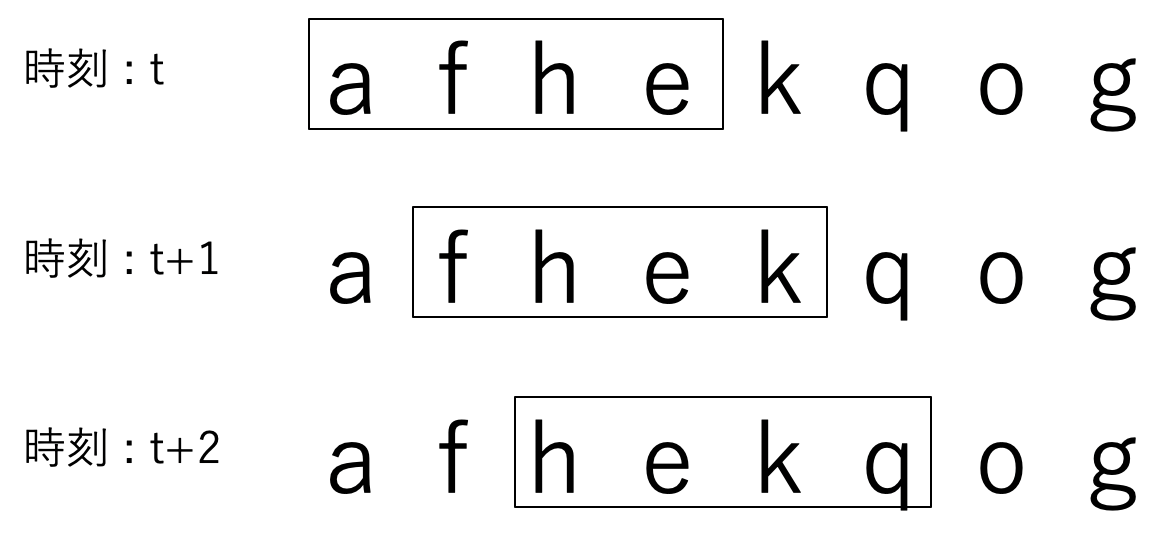
\includegraphics[width=15cm]{3_2_Ver1.1.png}
 \caption{スライディングウインドウ}
\label{fig:window}
\end{figure}

動的に変化する集合に対してハッシュ値を計算する自明な手法は,時刻経過によりウインドウがスライドするたびにハッシュ値を完全に
再計算するやり方である.これはすなわち,時刻が$t$から$t+1$に変化した際に,$h(A_{t+1})$を$A_{t}$とは無関係に計算するということ
である.この手法では,毎時刻ウィンドウ内の全要素をスキャンする必要があるので,$h(A_{t+1})$を求めるための時間計算量は$O(w)$
となる.

しかし、$A_t$と$A_{t+1}$は$e_t$と$e_{t+w}$以外の$w-1$個の要素が共通であり,$h(A_t)$計算時に判明した情報を再利用すること
で$h(A_{t+1})$を計算するオーバーヘッドを減らせる可能性がある.

\section{Datarらの手法}
Datar[1]らの手法の基本アイデアは
\begin{itemize}
\item 将来に割り当て値が最小になる可能性が絶対にない要素をあらかじめ削除することで,
次の時刻のハッシュ値$h(A_{t+1})$を計算する時に参照する要素数を減らす
\end{itemize}
というものである.ここで割り当て値が最小になる可能性が絶対にない要素とは,「ウィンドウ内で自分より後方に割り当て値が小さい要素が存在
する要素」のことである.例えば,$A_{t}$内の2要素$e_i$と$e_j$ ($i<j$)の割り当て値が$\pi(e_i)>\pi(e_j)$を満たすとしよう.
この時,$e_i$は自分より後方に割り当て値が小さい$e_j$が存在するという条件を満足する.この条件の下では$e_i$がウィンドウ内に存在する期間は$e_j$も必ずスライディングウィンドウ内に存在するので,$e_i$の割り当て値が最小になることはありえない(図\ref{fig:datar_ML} ).
Datarの手法ではこの性質を利用して,スライディングウインドウから最小値になりえない要素を削除し,将来最小値になりうる要素のみをMinlistというリストで管理する.
%Datarの手法ではこの性質を利用して,スライディングウインドウ内で将来最小値になりうる要素のリストMinlistを作成して管理する.
$A_t$のハッシュ値はMinlistに残った要素の割り当て値の最小値となる.
%\begin{equation}
 %\label{eq:datar}
%h(A_t)= \min_{e \in \mbox{Minlist}} \pi(e).
%\end{equation}
任意のMinlist内の要素$e$に対して,$e$より後方に割り当て値$\pi(e)$より小さい要素は存在しないので,
Minlist内の要素群に対する割り当て値は単調増加となる.このため,$h(A_{t})$は実はMinlistの先頭要素の
割り当て値と等しい.

\begin{figure}[H]
 \centering
 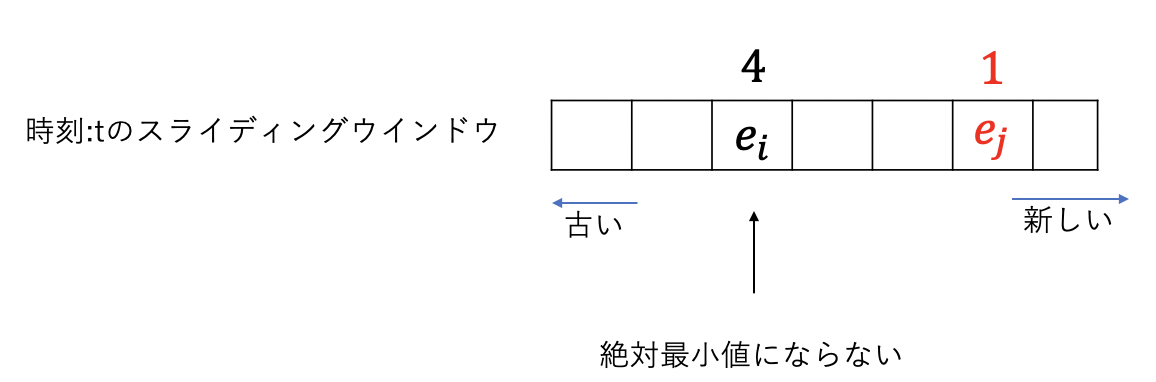
\includegraphics[width=15cm]{datar_ML.png}
 \caption{スライディングウインドウモデルの性質}
 \label{fig:datar_ML}
\end{figure}

時刻が$t$から$t+1$に変化した時にMinlistを更新する手順を以下にまとめる.
\begin{itemize}
\item $e_{t-w+1}$がウィンドウから離脱した時の処理\\
$e_{t-w+1}$がMinlistに含まれる時には$e_{t-w+1}$をMinlistから削除する.この時,$h(A_t)=\pi(e_{t-w+1})$であるため,ハッシュ値を更新する必要がある.そのため,$h(A_{t+1})$を新たにMinlistの先頭になった要素の割り当て値とする.
\item $e_{t+1}$をウィンドウに追加した時の処理\\
Minlist内で割り当て値が$\pi(e_{t+1})$より大きい要素は,今後,割り当て値が最小になりえないので削除する.
$e_{t+1}$によりMinlist内の他の要素がすべて削除された結果,Minlistに$e_{t+1}$のみ残った場合は
$h(A_{t+1})=\pi({e_{t+1}})$とする.
\end{itemize}


このアルゴリズムの動きを図 \ref{fig:koho2} に例示する.

%一番最初にスライディングウインドウからMinlistを作成する時は,前の要素から一つずつ見ていって,候補リストに加えていく.その過程で,加えた要素より前に自分より大きい要素があれば削除する.その工程を一番後ろの要素まで行うと単調増加の候補リストが作成される.これは候補リストの中で一番前の要素が一番小さく,Min-hashによるハッシュ値の値となるということである.そして,

時刻t+1の時,スライディングウインドウから一番前の要素$e_{t-w+1}$を削除し,新しい要素$e_t+1$のアルファベットkが入ってくる.kの割り当て値は3であるので,Minlistの中から3より大きい割り当て値を持つ要素を削除し,候補リストの一番後ろにkの割り当て値3を加える.
%つまり,スライディングウインドウ更新の際は,一番古い要素が候補リストに入って入れば削除し,新しい要素の割り当て値より大きい値が候補リストに存在する場合は,その中から削除する.そして,候補リストの一番後ろに新しい要素の割り当て値を加える.


\begin{figure}[H]
 \centering
 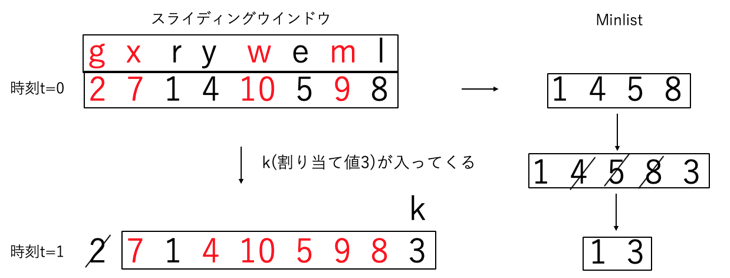
\includegraphics[width=15cm]{koho2.png}
 \caption{候補リストの作成}
 \label{fig:koho2}
\end{figure}

このようにDatarらは作成した最小値の候補リストを持ちいることにより,スライディングウインドウを保持する必要がない.そのため,ウインドウサイズWの場合, 候補リストは$\log(W)$で保持することができ,二部探索で候補リストを探索し,実行時間は$\log\log(W)$となることが保証される.

\chapter{多重集合に対するハッシュ値更新アルゴリズム}
本論文では,Datarらのアルゴリズムを動的に変化する多重集合に対して拡張したハッシュ値更新アルゴリズム
SWMH (Sliding-Window Min-Hash)を提案する.
Datarら[1]のアルゴリズムを多重集合に拡張する場合,スライディングウインドウ内の要素$e$への割り当て値が$e$と同じラベルを持つウインドウ内の要素数によって変化する点が難しくなる.つまり,$e$への割り当て値が時間経過によって変化することが起きる.
スライディングウインドウ内の要素$e$のラベルをアルファベット$l(e)$とする.割り当て値$\pi(e)$はスライディングウインドウ内に$l(e)$が何個あるかによって変わる.例えば,図\ref{fig:43}の場合だと,時刻$t=0$の時は,スライディングウインドウ内にアルファベット$b$は2つあり,$\pi(e_i)=4$, $\pi(e_j)$=1となる.時刻$t=3$でスライディングウインドウから要素$e_i$が抜けた場合,$e_j$への割り当て値$\pi(e_j)$は1から4に変化する.
\begin{figure}[H]
  \centering
  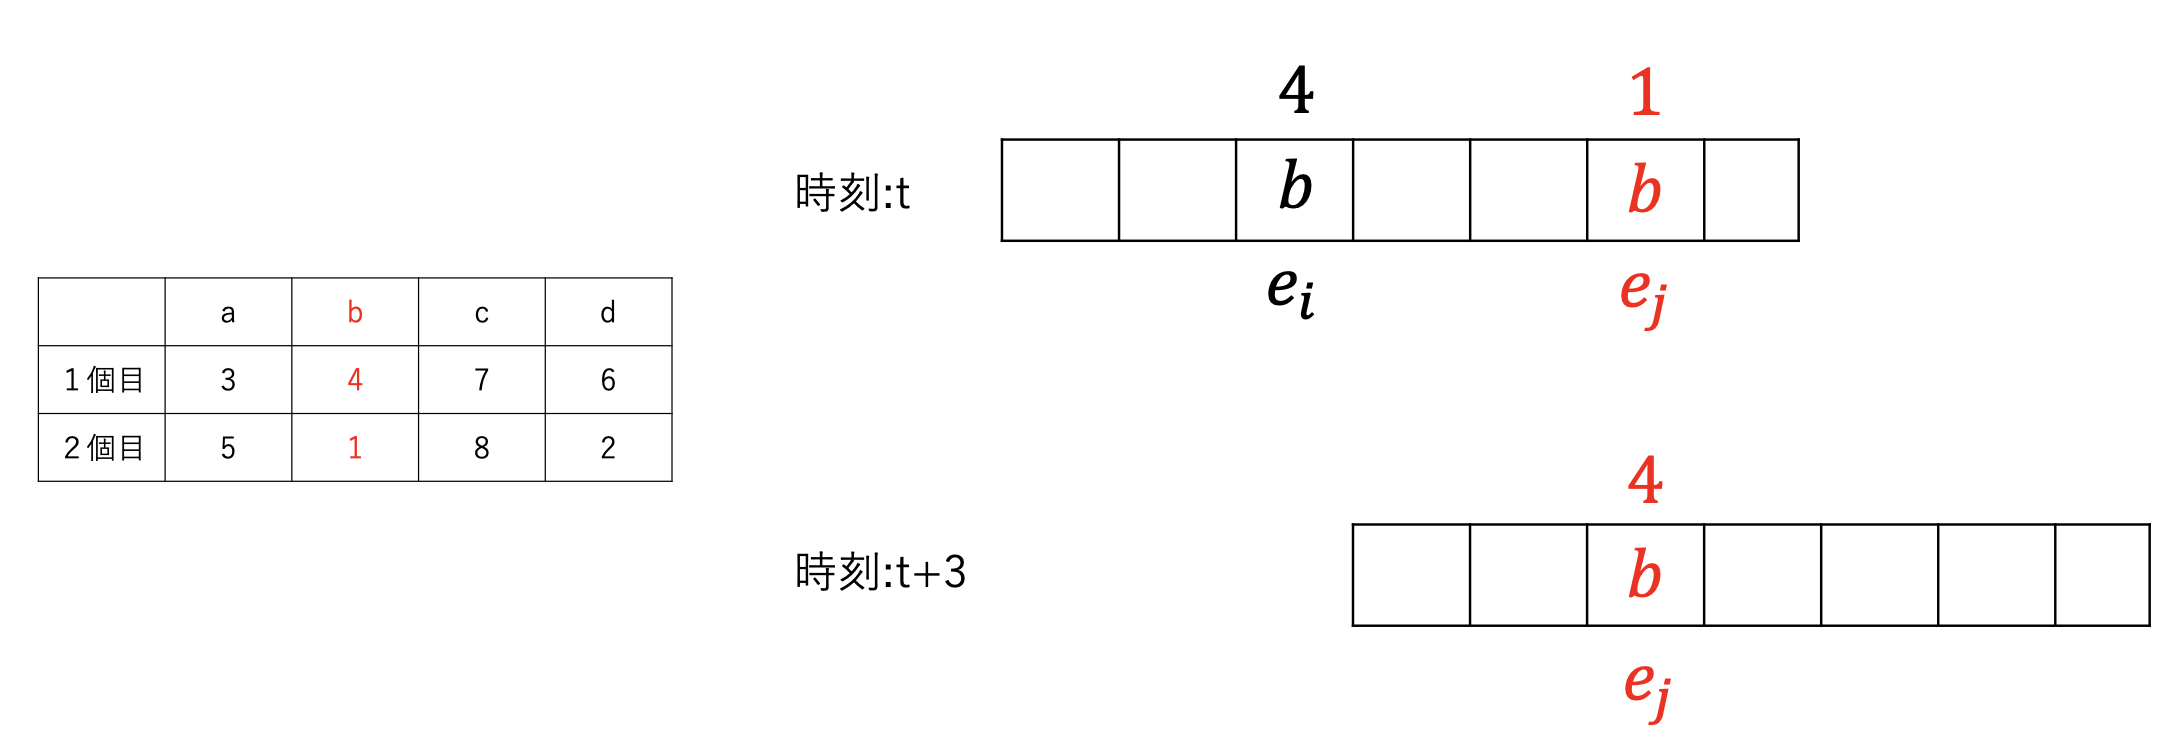
\includegraphics[width=18cm]{43.png}
    \caption{π(e)の変化}
    \label{fig:43}
\end{figure}
Datarらのアルゴリズムでは最小値になり得ない要素をMinlistから削除する.多重集合の場合,割り当て値が
変化することを考慮して最小値になり得るかどうかを判定をする必要がある.提案手法を基盤とする要素技術は
以下の2つであり,それぞれを順に説明する.
\begin{enumerate}
\item 同種アルファベットへの値の割り当て
\item スライディングウィンドウ更新時の処理
\end{enumerate}
%データストリームのスライディングウインドウ内の集合$A_t$が時刻経過により$A_{t+1}$に変化した時,
%R単純な手法は$A_t$を考慮しないでハッシュ値$h(A_{t+1})$を完全に再計算することである.しかし,多重集合に
%対してMin-Hashを何度も再計算をすることは多くの時間を必要とする.
%そして,$A_t$,$A_{t+1}$が多重集合ではなく集合であれば,2.1.2項で述べたDatar[1]らによる動的に変化する集合に対してハッシュ値の更新をするアルゴリズムにより,$h(A_t)$を$h(A_{t+1})$に更新することによって効率よくできる.しかし,このアルゴリズムは多重集合には対応していない.そこで,本研究では,集合に対応しているDatarらのアルゴリズムを多重集合に拡張したSWMHアルゴリズムを提案する.
%\subsection{多重集合の難しさ}
%SWMHではスライディングウインドウの中に同一種のアルファベットが複数存在する場合は到着時刻順に順番を決めている.
\section{同種アルファベットへの値の割り当て}
多重集合に対するMin-Hashでは,多重集合内に同種アルファベットが複数存在する場合それらを区別
して値を割り当てる.例えば,ラベルが$a$のアルファベットが$n$個存在する場合,それらを
$\{a_1,a_2,\cdots,a_n\}$のように区別する.$a_i$ ($1\le i \le $)は$i$番目の$a$という意味であり,
各$a_i$ ($1\le i \le n$)に異なる値$\pi(a_i)$を割り当てる.

ここで$\pi(a_i) \le \pi(a_{i+1})$ならば,$a_{i+1}$の割り当て値は最小には絶対ならない.その理由は
$i+1$番目の$a_{i+1}$が存在する条件下では,$i$番目の$a_{i}$も必ず存在するからである.このように
割り当て値$\pi(a_{i+1})$はMin Hashのハッシュ値に影響を与えないので
$$\pi(a_i) \le \pi(a_{i+1})$$
を条件を満足する限りは別の値に変更しても構わない.そこで,$\pi(a_i) \le \pi(a_{i+1})$が成立する場合は
$\pi(a_{i+1})$を$\pi(a_{i})$に修正する.修正前と修正後を区別するため,修正前の割り当て値を
$\pi(a_{i+1})$とし,修正後の割り当て値を$\pi'(a_{i+1})$とする.

%for文を使ったアルゴリズムの記述と説明。単調減少になることも述べる。Lemma1も載せる。

次にスライディングウィンドウ内の$n$個の$a$のインスタンスをそれぞれ何番目の$a$とするかを
考える.つまり,$n$個の$a$のインスタンスのインデックスをどう定めるかという問題である.
通常の多重集合であれば要素間に時間順序がないのでこの問題は重要でない.しかし、スライディング
ウィンドウの場合,要素間に時間順序があるためインデックスの決め方によって挙動が変わる.自然な
方式としては以下の2つが考えられる.
\begin{itemize}
\item 一番古い要素を$a_1$とし,$a$のインデックスを到着時刻の昇順とする
\item 一番新しい要素を$a_1$とし,$a$のインデックスを到着時刻の降順とする
\end{itemize}

提案手法では,「一番古い要素を$a_1$とし,$a$のインデックスを到着時刻の昇順とする」
という方式を採用する.この時,
\begin{enumerate}
\item $a_i$は$a_{i+1}$より先にデータストリームに到着した
\item $\pi(a_i)\ge \pi(a_{i+1})$
\end{enumerate}
が成立するため,$a_i$は$a_{i+1}$の存在によってMinlistから削除される.
このことが任意の$i$に対して成立するのので,以下のlemma\ref{le:lemma1}が保証される.
%このことが任意の$i$に対して成立するので,Minlistの中に同種アルファベットは最新の1要素しか存在しない事を保証できる.
\begin{lemma}
  \label{le:lemma1}
  Minlistの中に同種アルファベットは最新の1要素しか存在しない.
  \end{lemma}


\begin{lemma}
  \label{le:lemma2}
   $$\min\{\pi(a_1),\pi(a_2),\cdots,\pi(a_n)\} = \min\{\pi'(a_1),\pi'(a_2),\cdots,\pi'(a_n)\}$$
  \end{lemma}



また,lemma \ref{le:lemma2}
が成立するため割り当て値の修正によってハッシュ値は不変である.実際には多重度の上限値$n$をパラメータとして$\pi'$を保持する表を事前計算し,スライディングウィンドウに到着した要素の割り当て値は表を参照して決定する.割り当て表の修正例を図 \ref{fig:44}に示す.この例では多重度の上限が$n=2$であり,2個目の割り当て値が1個目より大きい場合,割り当て値を1個目と同じ値に書き換えている.また,ラベルが$c$の要素$e_i,e_j$の割り当て値の最小値は修正後も修正前から不変になっている.
動的多重集合の場合は,
書き換えによって,Minlistの同じアルファベットの前側の値を消せて,MInlistのサイズを小さくすることができる.




\begin{figure}[H]
  \centering
  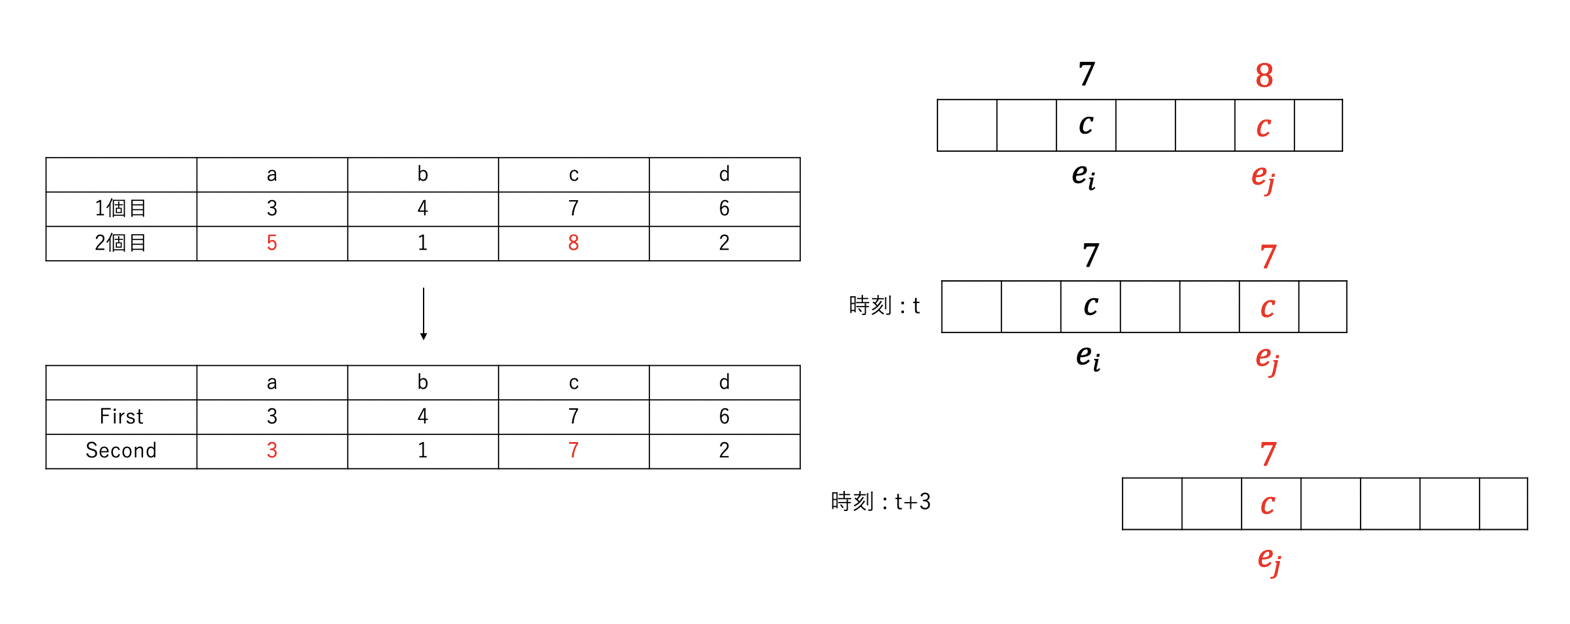
\includegraphics[width=18cm]{44.png}
    \caption{割り当て値の修正}
    \label{fig:44}
\end{figure}
%アルファベットの多重度の上限値が一般に$n(\geq2)$の場合,割り当て表は以下のように1つずつ各アルファベットに対して更新する.
%アルファベットαとする.π($α_1$)よりπ($α_2$)の方が少ない場合もあるが,逆にπ($α_1$)がπ($α_2$)より大きい場合もある.π($α_2$)が小さい場合は,どちらのも値も現在もしくは将来的にハッシュ値になる可能性があるので必要であるが,π($α_2$)が大きい場合,将来的に必要となることがないため,図4.2のようにπ($α_2$)をπ($α_1$)と同じ値で保持する.これは$i$番目でも同じように考えることができ,表にπ($α_i$)を登録する時,π($α_{i-1}$)より大きいか小さいかで上の説明と同じように登録する.
以降では記述を単純化のため,修正後の値割り当て$\pi'$を単に$\pi$と記載する.
\section{ヒストグラムの作成}
%多重集合のスライディングウインドウにおいてMin-hashを更新する場合,
スライディングウインドウが多重集合である場合,スライディングウインドウ内にいくつ同一要素が含まれているかわからないとMin-hashのハッシュ値を計算できない.そこで要素のヒストグラムを保持する.さらに各要素の到着時刻も保持するためヒストグラムのビンを到着時刻のリストとして管理し,リストのサイズにより各アルファベットのスライディングウインドウ内の個数を取得する(図 \ref{fig:4_3_2}).リストは到着時刻が昇順で保持され,新たにウィンドウに到着した要素の到着時刻がエンキューされ,ウインドウから出ていく要素の到着時刻がデキューされる.
%そして,最小値候補リストであるMinlist更新のために,要素がスライディングウインドウに入ってきた時刻とスライディングウインドウ内の要素の個数の2つの情報が必要となる,この2つの情報を保持するために,ヒストグラムは要素の入ってきた時刻をヒストグラムに追加していくように作成した.この作成によって,ヒストグラムの中身で時刻を判断し,ヒストグラムの個数で要素の個数を判断することができる.(図 \ref{fig:4_3_2})
\begin{figure}[H]
  \centering
  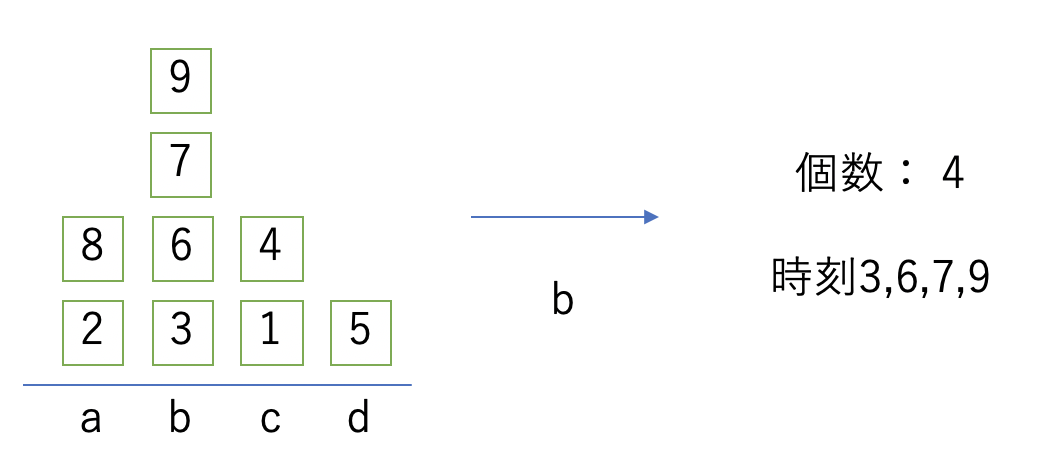
\includegraphics[width=15cm]{4_3_2.png}
    \caption{ヒストグラム}
    \label{fig:4_3_2}
\end{figure}
\subsection{スライディングウインドウの更新}
提案手法SWMHでもDatarらの手法と同様に最小値になりうる要素のリストMinlistを管理する.DatarらのアルゴリズムではMinlistに割り当て値のみを保持していた.
しかし多重集合の場合,割り当て値が変化が発生すると現在の割り当て値から変化後の値を計算できない.変化後の値を計算するため,Minlistは
\begin{itemize}
\item 現在の割り当て値 : $\pi(e)$
\item 要素のラベル : $l (e)$
\item 要素の到着時刻 : $t(e)$
\end{itemize}
の3つ組を要素とするリストとする.
さらにSWMHでは多重集合$A_t$が$A_{t+1}$に変化する時,(1)ウィンドウから一番古い要素$e_{t-w+1}$が離脱する時の
処理と(2)ウインドウに新要素$e_t$に入ってくる時の処理を拡張しなくてはいけない.
%Minlistに.
%しかし,集合の時のように単調増加のリストにはならないため,更新の際に,手間は多くなる.そして,多重集合で行う場合,
\subsection{要素$e_{t-w+1}$がウィンドウから出ていく処理}
%Minlist内で最小割り当て値となる要素$\alpha$のアルファベットを$x$と記述する.
時刻$t$に割り当て値が最小値でハッシュ値と対応する要素を$\alpha$とし,そのラベルを$l(\alpha)$とする.
\noindent (Case 1): Minlistの先頭要素の時刻が$t-w+1$ならばMinlistの先頭要素は$e_{t-w+1}$そのものなのでデキューする.この時,$l(e_{t-w+1}) = l(\alpha)$であったとする.$lemmma$\ref{le:lemma1}より,Minlist内に同じラベルを持つ要素は複数存在しないので$e_{t-w+1}$は$\alpha$と一致する.つまり,ハッシュ値と対応する要素が離脱するため,ハッシュ値の更新が必要となる.
$\alpha$がウィンドウから離脱することになる.そこで,新たに最小割り当て値となる要素をMinlistから探索して更新する.Minlistは割り当て値順にソートされていないので,この操作は
Minlistの全要素のスキャンを伴う.

\noindent (Case 2): Minlistの先頭要素の時刻が$t-w+1$でない場合は$e_{t-w+1}$はMinlistのメンバーではないためMinlistからのデキューは不要である.
しかしこの場合もMinlist内で最小割り当て値が変化する場合がある.具体的には離脱要素$e_{t-w+1}$のアルファベット
が$l({\alpha})$である場合,$l(\alpha)$の多重度が1減るため$\alpha$の割り当て値が増加し,$\alpha$の割り当て値が
ウィンドウ内で最小でなくなる可能性がある.この場合もMinlistをスキャンし新たな最小割り当て値を
探索する.
Case(2)で$e_{t-w+1}$のアルファベットが$l(\alpha)$でない場合,最小割り当て値は不変である.しかし,
Minlist内にラベルが$l(e_{t-w+1})$の要素$\beta$が存在した場合,$\pi(\beta)$は同じラベルの要素数が減少しすることに伴い本来増加する.
しかし,最小割り当て値には影響を与えないのでMinlist内では$\beta$の割り当て値を更新しない.
この結果,Minlist内に保持されている$\beta$の割り当て値は(一時的に)不正確になる.
不正確になった割り当て値の修正は,(Case 2)で最小割り当て値をMinlistをスキャンして更新するときに同時に行う.
正しい割り当て値は$\beta$のアルファベット$l(\beta)$の多重度をヒストグラムから得ることで算出できる.
%先頭要素の時刻が$t$ならば
% アルファベット$x$がMinlistを更新する.最小値の要素がウインドウから出ていく時以外にMinlistを更新しないことによって,Minlistに本来と違う割り当て値で保持される.しかし,割り当て表が単調減少であるため,最小値の選択に影響はなく,毎時刻Minlistを確認する必要がなくなる.間違えている値は,最小値のアルファベットと同じアルファベットがウインドウから出ていく時に一緒に修正する.
% インドウから出ていく時,以下のようにMinlistを更新する.
%
%\begin{itemize}
%\item Minlistの先頭の要素$e_{t+a} (0 \leq a \leq w-1)$,現在の時刻$t_n$,スライディングウインドウの長さ$w$とする.時刻$t(e_{t+a})$と$t_n-w$が一致するならば,Minlistから$e_{t+a}$を削除する.
%\item 現在のハッシュ値を持つ要素のアルファベットとxが一致する場合,Minlistの間違っている割り当て値を修正しつつ,最小値を現在のMinlistの最小値に更新する.
%\end{itemize}
 \subsection{要素$e_{t+1}$をウィンドウに入る時の処理}
$e_{t+1}$がスライディングウインドウに入る時に,Datarらの手法ではMinlistの中で$\pi(e_{t+1})$より
割り当て値が大きい要素を消すだけで十分だった.
しかし,多重集合の場合は$\pi(e_{t+1})$が将来増加する可能性があり,単に$\pi(e_{t+1})$より割り当て値が大きい要素を消すと割り当て値が最小となる可能性がある要素も消してしまう.
そこで,$\pi(e_{t+1})$ではなく,$e_{t+1}$の将来の割り当て
値の上限を上回る要素だけ削除する.$e_{t+1}$のアルファベットを$l(e_{t+1})$とする.
また,Minlist内の要素$\gamma$の到着時刻を$t_{\gamma}$として,$t_{\gamma}$よりあとに到着した
アルファベット$l(e_{t+1})$の個数を$n$とする.$n$の値はヒストグラムの$l(e_{t+1})$のビンに記録された到着時刻
のリストを後方から前方にスキャンすることで求められる.この時,
$$\pi(l(e_{t+1})_{n})<\pi(\gamma))$$
であれば,要素$\gamma$をMinlistから削除してよい.
最後にMinlistの一番後ろに$e_{t+1}$を挿入し,$\pi(e_{t+1})$がMinlistの最小値を更新するかをチェックする.
アルゴリズムの動きをAlgorithm 1に示す.
\begin{figure}[H]
  \centering
  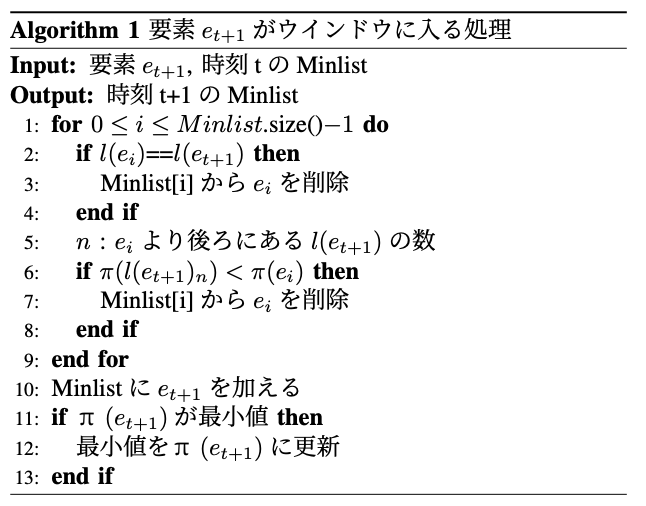
\includegraphics[width=12cm]{4_2_3.png}
    \label{fig:423}
\end{figure}
%e_{w+1}$と同じアルファベットである$\alpha$のスライディ
%ングウインドウ内の個数$n$,割り当て値$\pi$として,$e_{\beta}$よりあとに
%到着した$\alpha$の個数に応じた$\pi$により,将来的に最小値になり得るかど
%うか判断する.以下の処理でMinlistを更新する.

%\begin{figure}[H]
 % \centering
  %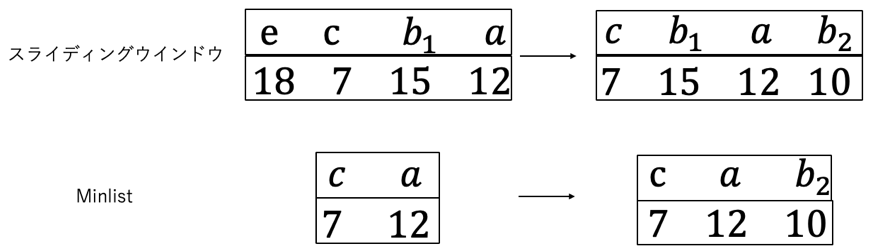
\includegraphics[width=9cm]{45.png}
   % \caption{Minlistの更新}
%\label{fig:minlistupdate}
%\end{figure}
%図\ref{fig:minlistupdate}にMinlistの更新例を示す.


\chapter{バッチSWMH}
前章で説明したSWMHでは,データストリームに毎時刻要素が1つだけ到着することを仮定したが,現実のデータストリームでは,1度に複数個の要素が到着することも普通である.そこで,そのような場合にSWMHを拡張することを目指す,本章では,データストリームに毎時刻$c$個の要素が到着するモデルを想定する.
%私たちは,4節で紹介したSWMHをスライディングに毎時刻複数個の要素が出入りする場合に対応するMinlist更新アルゴリズムであるバッチSWMHを開発した.


\section{自明な手法}
データストリームに毎時刻$c$個の要素が到着するモデルにおいての自明な手法は,4章で説明したSWMHを$c$回適応する手法である.つまり,スライディングウインドウが$c$回ずれる事象を,スライディングウインドウが1つずれる事が$c$回繰り返されると判断して,SWMHを$c$回適用する,1回SWMHを適用する度にMinlistが1回適用されるので,1時刻あたり$c$回Minlistをスキャンすることになる.


\begin{figure}[H]
  \centering
  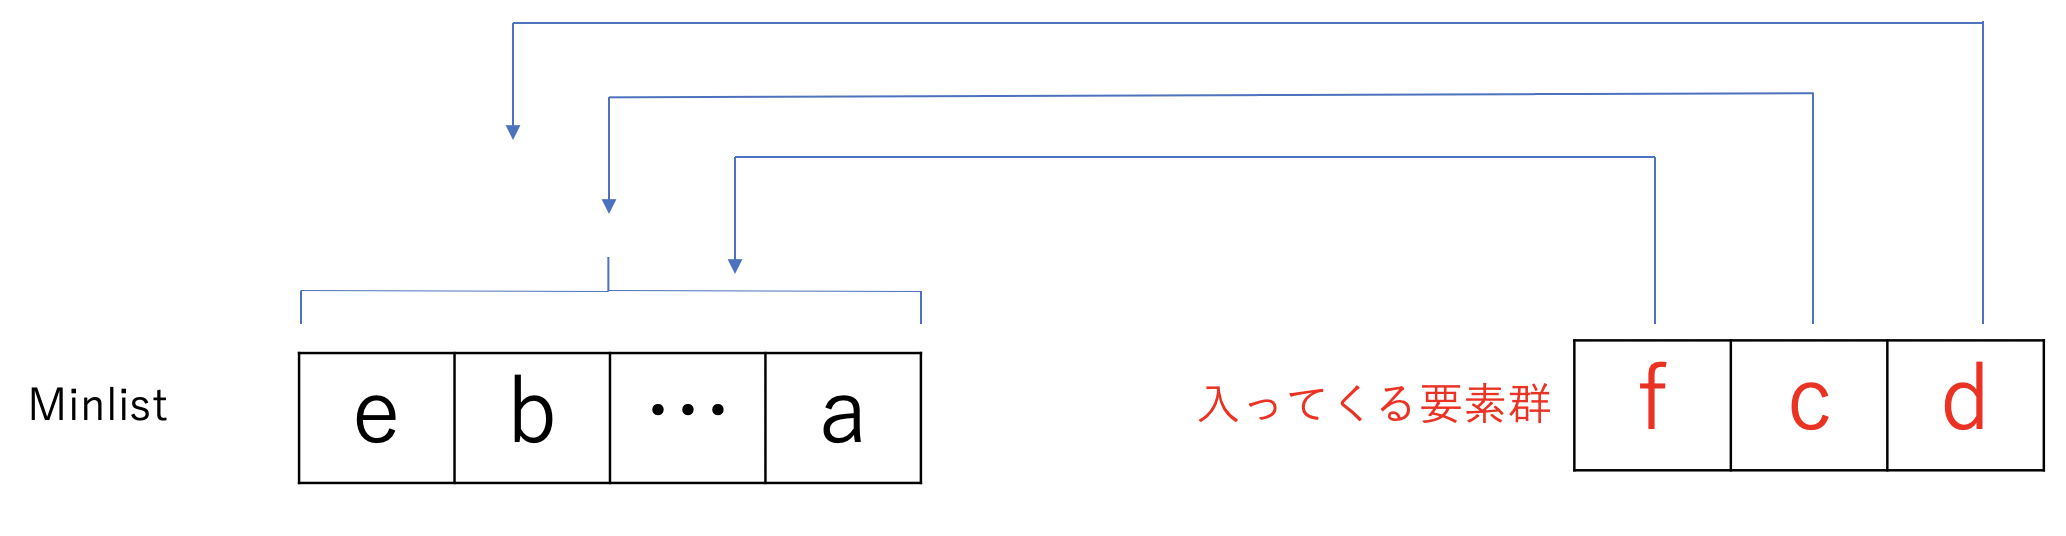
\includegraphics[width=15cm]{6_1.png}
    \caption{Minlistの更新}
\end{figure}

\section{バッチSWMHのアルゴリズム}
本章ではMinlistを$c$回スキャンせず1回だけスキャンするバッチSWMHを提案する.
バッチSWMHのアルゴリズムでは,ウインドウから要素が出ていく場合と入ってくる場合に処理を分けて考える.ウインドウにc個の要素が出入りする場合,ウインドウから出ていく要素群を$E_{t-w/c+1} = $\{$e^1_{t-w/c+1},e^2_{t-w/c+1},...,e^c_{t-w/c+1}$\},入ってくる要素群を$E_{t} = $\{$e^1_t,e^2_t,...,e^c_t$\}とする.

\subsection{要素群$E_{t-w/c+1}$が出ていく処理}
バッチSWMHの$E_{t-w/c+1}$が出ていく処理では,4.2.1節のSWMHのウインドウから要素が出ていく時に対する処理と同じように場合分けをして処理を行う.Minlist 内で最小割り当て値となる要素$\alpha$のアルファベットを$x$と記述する.

\noindent (Case1):Minlistの先頭要素の時刻が$t-w/c+1$ならばMinlistの先頭要素をデキューする.さらに,Minlistの要素が$t-w/c+1$と違う時刻要素が出てくるまでMinlistをスキャンし,$t-w/c+1$と同じ時刻を持つ要素を削除する.この時,削除される要素が$\alpha$と同じアルファベット$x$を持つ場合,新たな最小割り当て値となる要素をMinlistから探索して更新する.Minlistは割り当て値順にソートされていないので,この操作はMinlistの全要素のスキャンを伴う.

\noindent (Case2):Minlistの先頭時刻が$t-w/c+1$でない場合,Minlistからのデキューは不要である.不要である理由は,4.2.1節で説明した理由と同じである.


\subsection{要素群$E_t$が入ってくる処理}
Minlistに$E_t$が入ってくる処理では,以下の3つの手順で行う.
\begin{itemize}
\item $E_t$から代表アルファベットの選択
\item 代表アルファベットと比較して,Minlistをスキャン
\item Minlistへ$E_t$を追加

代表アルファベットとは,$E_t$の中で割り当て値が最小のアルファベット$x$と$E_t$の中でスライディングウインドウ内の多重度最大のアルファベット$y$である.

そして,Minlistのスキャンでは,$E_t$内の要素と同じラベルの要素の削除と違うラベルの削除の2つの処理を行う.Minlistの要素を$\lambda$とする.
(1) $E_t$内の要素と同じラベルの要素の削除

同じアルファベットを消すために,従来の手法では,$\lambda$に対して,$E_t$全体をスキャンし,同じアルファベットが複数存在するか確認する必要があった.しかし,私たちは先に保持させたヒストグラムの情報の1つである時刻を用いて,ヒストグラムの最後尾に入っている要素の時刻と$l(\lambda)$の時刻を比較することで,同じアルファベットの中で一番最後尾の要素のみを残し,ほかの要素を削除することができる.

 (2)$E_t$内の要素と違うラベルの要素の削除
$E_t$の中で,$x$,$y$の2つのアルファベットを用いてスキャンを行なっていく.Minlist内の要素$\lambda$の入ってきた時刻$t_\lambda$とし,$t_\lambda$よりあとに到着した$x$, $y$の個数$n_x$,$n_y$とする.時刻に応じて,$x$,$y$のうち小さい割り当て値を持つアルファベットの割り当て値を用いて,Minlistから将来の割り当て値の上限を上回る要素を削除していく.

\begin{quote}
$\pi_{{\rm min}} = {\rm min}(\pi(x_{n_x}),\pi(y_{n_y}))$ \\
 {\bf if} ($\pi_{{\rm min}}<\pi(l(\lambda))$)  Minlistから $\lambda$を削除\\
\end{quote}
% まず,$E_t$の要素すべてヒストグラムに追加する.始めにヒストグラムに追加することを利用して,以下の3つの手順で処理を行う.


%\subsubsection{ \scalebox{1.2}{手順1:要素群の更新と代表アルファベットの選択}}
%$E_t$を後ろからスキャンし,将来最小値になり得ない要素の削除と,Minlistをスキャンする際の基準アルファベットの選択を行う.基準アルファベットとは,$E_t$の中で割り当て値が最小のアルファベット$x$と$E_t$の中でスライディングウインドウ内の多重度最大のアルファベット$y$である.
%$c$個の要素群が入ってくることに対して,その中の1つのアルファベットだけでMinlistをスキャンより,2つのアルファベットを使う方が割り当て値の変化により対応でき,Minlistを短く保つことにつなるために,基準アルファベットを2つ選択する.
%スキャンされる側の$E_t$内の要素を$e^z_t (1 \le z<c)$,$E_t$の一番最後尾の要素$e^c_t$のラベルのアルファベットを $x = l(e^c_t)$,$y = l(e^c_t)$として,後ろから順に以下の処理を行なっていく.

%(1) $e^z_t$と同じアルファベットが$E_t$内に複数存在するか確認

 %$e^z_t$と同じアルファベットを消すために,従来の手法では,$E_t$全体をスキャンし,同じアルファベットが複数存在するか確認する必要があるため,$O(c)$の時間を要する.しかし,私たちは先に保持させたヒストグラムの情報の1つである時刻を用いて,ヒストグラムの最後尾に入っている要素の時刻と$e^z_t$の時刻を比較することで,同じアルファベットの中で一番最後尾の要素のみを残し,ほかの要素を削除することができる.
 
 %(2)違うアルファベットの中で必要ない要素の削除とx,yの更新
 %$\pi(e^z_t)$より$\pi(x)$が大きい場合, $e^z_t$を削除し,小さい場合$x$を更新する,さらに,$e^z_t$のアルファベットが$E_t$内でヒストグラム最大の場合,$y$を更新する.

%\begin{quote}
%{\bf if} ( $\pi(x) \le \pi(e^z_t)$ )\{ \\
%\hspace*{1cm} $e^z_t$を$E_t$から削除する.\\
%\}
%{\bf else}  $x = \l(e^z_t)$  \\

%{\bf if} ( ${ \rm histgram}(y).{\rm size} < { \rm histgram}(\l(e^z_t)).{\rm size}$ ) $y = \l(e^z_t)$

%\end{quote}


%\begin{equation}
 %\label{eq:5_2}
%x = \l(e^a_t) \; \; \; (1\le a \le c-1)
%\end{equation}\

%(3)入ってきた要素群$E_t$から将来最小値になり得る要素のみを残した要素群$E'_t$として保持する.


%\subsubsection{ \scalebox{1.2}{手順2:Minlistのスキャン}}
%手順2では,Minlist内で手順1と同じように$E'_t$の要素のアルファベットと同じ要素の削除と,将来最小値になり得ないアルファベットを持つ要素の削除を行なっていく.同じアルファベットの要素の削除は,手順1の方法により,ヒストグラムを利用して削除していく.
%将来最小値になり得ないアルファベットを持つ要素の削除するために,$E_t$の中で,$x$,$y$の2つのアルファベットを用いてスキャンを行なっていく.Minlist内の要素$\lambda$の入ってきた時刻$t_\lambda$とし,$t_\lambda$よりあとに到着した$x$, $y$の個数$n_x$,$n_y$とする.時刻に応じて,$x$,$y$のうち小さい割り当て値を持つアルファベットの割り当て値を用いて,Minlistから将来の割り当て値の上限を上回る要素を削除していく.

%\begin{quote}
%$\pi_{{\rm min}} = {\rm min}(\pi(x_{n_x}),\pi(y_{n_y}))$ \\
 %{\bf if} ($\pi_{{\rm min}}<\pi(l(\lambda))$)  Minlistから $\lambda$を削除\\
%\end{quote}



\subsubsection{ \scalebox{1.2}{手順3:Minlistへの追加}}
最小値となり得ない要素を削除したMinlistに対して,$E'_t$を追加する.

%\begin{quote}
%{\bf if} ($   \pi(y_{n_x}) \le \pi(y_{n_y})$)\{ \\
%\hspace*{1cm} {\bf if} ($\pi(a_{i+1})>\pi'(a_i)$) $\pi'(a_{i+1})=\pi'(a_i)$ \\
%\hspace*{1cm} {\bf else} $\pi'(a_{i+1})=\pi(a_{i+1})$ \\
%\}
\chapter{実験}
本章では提案手法であるSWMHと,バッチSWMHを人工データと実データを用いて実験的に評価する.6.1節で使用したデータセットを記述する.次に,6.2節ではデータストリームの到着レートが1である状況でSWMHを評価する.ここでは,時刻変化のたびにスライディングウインドウ全体をスキャンして,Min-hashのハッシュ値を再計算する手法をBaselineとし,SWMHがBaselineより高速であることを示す.6.3節ではデータストリームの到着レートが$c>1$である条件でバッチSWMHを評価する.ここでは,5.1節で述べたSWMHを$c$回適用する単純手法とバッチSWMHの実行時間を比較する.





\section{データセット}
\subsection{人工データセット}
人工データセットは,アルファベット$\phi$から,zipf分布に従ってサンプリングを繰り返し,長さ100,000の文字列$st$を生成する.
到着レートを$c$として,データストリームは$st$の先頭から順に毎時刻$c$個取り出すことで,シミュレートする.データセットの特性を決定するパラメータは
\begin{itemize}
\item $\alpha$ : zipf分布の偏りをコントロールするパラメータ
\item $\phi$ :アルファベットの種類数
\end{itemize}

であり,スライディングウインドウのの長さを $W$とする.
zipf分布とは,$\alpha$を$[0,1]$の範囲で指定し,アルファベットの出現頻度に偏りを持たせた分布である.アルファベットの出現順位を$k$,$k$番目のアルファベットの個数を$N_k$,一番出現頻度の高いアルファベットの個数を$N_{max}$とすると,zipf分布は以下の式\ref{eq:zipf}で表せる.

\begin{equation}
 \label{eq:zipf}
N_k = N_{max} \times 1/k^\alpha
\end{equation}

$\alpha$はzipf分布の偏りをコントロールするパラメータで$\alpha$が大きいほど出現頻度の偏りが大きい.その結果,$\alpha$が大きいほどスライディングウインドウ内の要素の多重度大きくなる.$\alpha = 0$の時は単に一様分布に従ってサンプリングがなされる.

\subsection{実データセット}
実データによる実験は,connect datasetとmushroom datasetの2種類のデータ \cite{Maxloghash} \cite{dataset2} からデータベースを作成した.まず,connect datasetとは117種類のラベルが出現し,約20の長さのラベルから成る集合が約4,000列連なったデータである.次に,mushroom datasetとは127種類のラベルが出現し,約20の長さのラベルから成る集合が約60,000列連なったデータである.どちらのデータも1つの集合に同じラベルは含まれないデータである.それらのデータからランダムに集合を1つ選ぶ処理を,選ばれた集合をつなげた長さがデータストリームの長さ$100,000 + $ウインドウサイズ $W$を超える長さになるまで行い,データストリーム$st$を生成する.人工データと同じように,到着レートを$c$として,データストリームは$st$の先頭から順に毎時刻$c$個取り出すことで,シミュレートする.

\section{SWMHの実験評価}
まず,人工データを使った評価主数を説明する.人工データのパラメータは以下の3つである.
\begin{itemize}
\item $\alpha$
\item $\phi$
\item $W$

\end{itemize}

$\alpha = 1$, $|\phi|=100$,$W = 100$という組み合わせをデフォルトパラメータとし,それぞれのパラメータを変更し,実験を行なった.

次に,実データを使った評価主数を説明する.実データのパラメータは,

\begin{itemize}
\item $W$
\end{itemize}

のみであり,$W = 100$をデフォルトパラメータとし,実験を行なった.

それぞれの実験において,実験のばらつきを減らすために,ハッシュ関数を10個生成し,SWMH10回の合計を実行時間とし,実験を行なった.


実験	1): ウインドウサイズ $W$を変えて実験

スライディングウインドウサイズ $W = 100, 500, 1000, 5000, 10000$と変えて,提案手法の実行速度と最小値候補リストMinlistの長さを計測した.
人工データ, connect, mushroomいずれのデータセットにおいても,SWMHがBaselineより圧倒的に早かった(図\ref{fig:jikken1_1},\ref{fig:jikken1_2} ,\ref{fig:jikken1_3}).SWMHの実行時間は,Baselineと比べて,W=100の時,約9倍,W=1000の時,約17倍,W=10000の時,約60倍となった.実行時間とWの関係をより詳しく調査するため人工データに対する実行時間を対数グラフで表現したものを図\ref{fig:jikken1_taisu}に表す.Baselineでは,実行時間がWに対してリニアに増加するのに対して,SWMHでは実行時間が$\log (W)$に比例して増加する.Baselineの実行時間が$W$に比例するのはMin-hashの計算時間がO$(W)$であるためである.一方,SWMHの実行時間はMinlistの長さに関係があると考えられる.そこでMinlistの長さを調べた結果を図\ref{fig:jikken1_ML}に表す.Minlistの長さは,毎時刻ごとのMinlistの長さの1時刻の平均を表している.

%スライディングウインドウサイズ $W = 100, 1000, 10000$と変えて,提案手法の実行速度と最小値候補リストMinlistの長さを計測した. 割り当て値は,5回ランダムに生成し,実行速度とMinlistの計測は5回の平均値である.

%結果は,図\ref{fig:jikken1_1},\ref{fig:jikken1_2} ,\ref{fig:jikken1_3}より,人工データ,connect dataset, mushroom datasetのいずれのデータでも,Baselineではウインドウが長くなるごとに,大幅に実行時間が伸びていき,$W=10000$の時は,$W=100$の時に比べて,約50倍ほどの時間がかかっていることがわかる.図\ref{fig:jikken1_ML}より, 提案手法では,$W=10000$の時,$W=100$の時に比べて,約5倍ほどの時間で実行できており,$W$が大きくなっても,Baselineより与えられた影響が少ないことがわかる.


\begin{figure*}[h]
    \begin{tabular}{cc}
      %---- 最初の図 ---------------------------
      \begin{minipage}[t]{0.5\hsize}
        \centering
        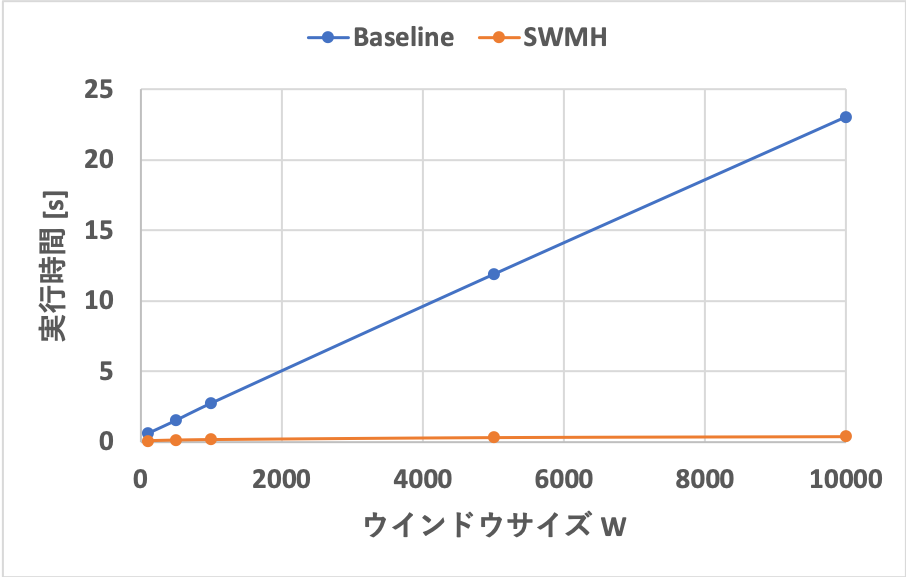
\includegraphics[width=8cm]{SW_jinko.png}
        \caption{人工 dataset}
        \label{fig:jikken1_1}
      \end{minipage}
      %---- 2番目の図 --------------------------
         \begin{minipage}[t]{0.5\hsize}
        \centering
        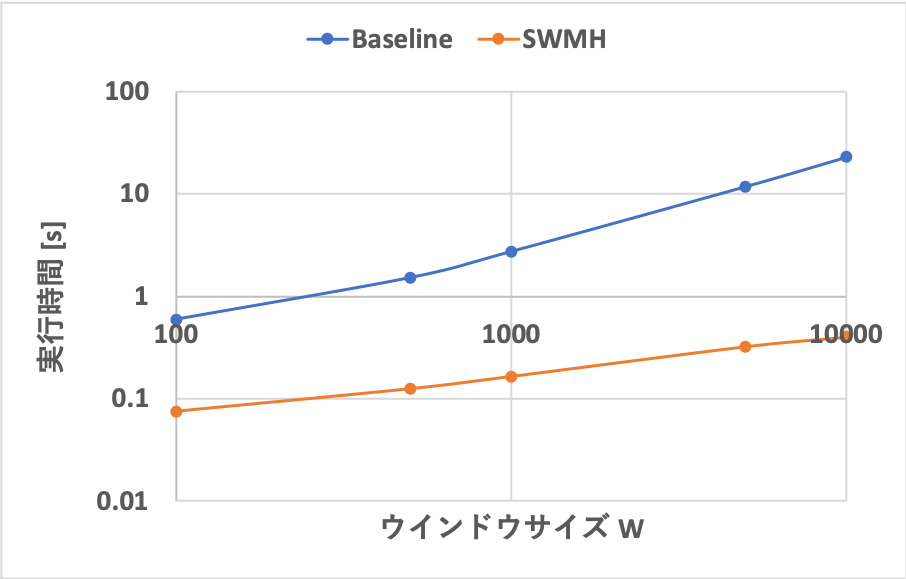
\includegraphics[width=8cm]{jikken1_1_taisu.png}
        \caption{人工datasetにおける対数グラフ}
          \label{fig:jikken1_taisu}
      \end{minipage}
      %---- 図はここまで ----------------------
    \end{tabular}
  \end{figure*}
  
   % \begin{figure*}[t]
  %\centering
  %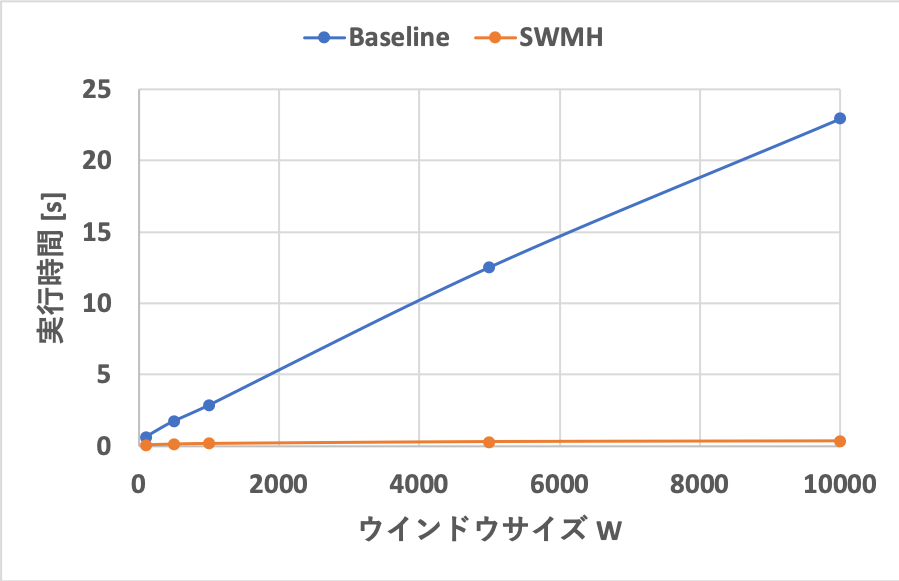
\includegraphics[width=8cm]{SW_connect.png}
    %\caption{connect dataset}
    %\label{fig:jikken1_3}
%\end{figure*}

\begin{figure*}[h]
    \begin{tabular}{cc}
      %---- 最初の図 ---------------------------
  \begin{minipage}[t]{0.5\hsize}
        \centering
        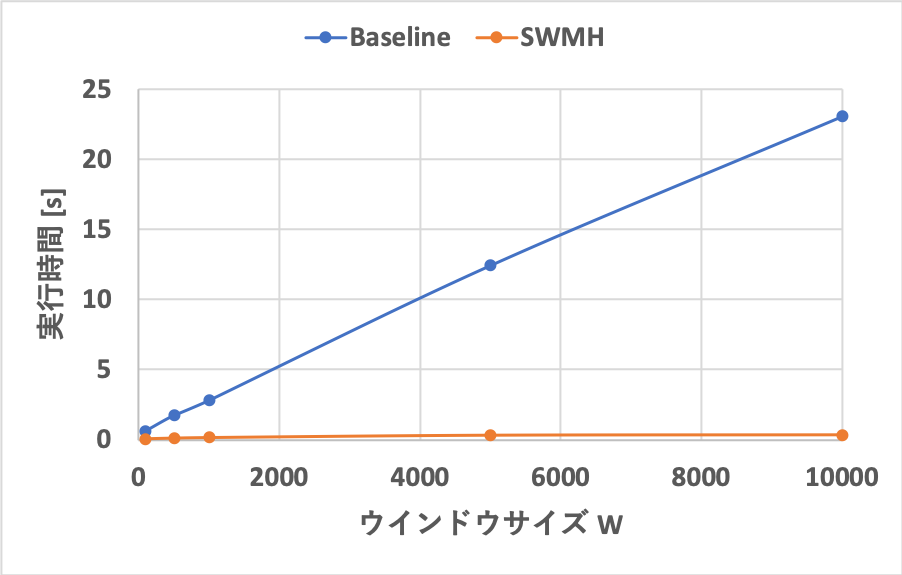
\includegraphics[width=8cm]{SW_mush.png}
        \caption{mushroom dataset}
          \label{fig:jikken1_2}
      \end{minipage}

      %---- 2番目の図 --------------------------
          \begin{minipage}[t]{0.5\hsize}
        \centering
        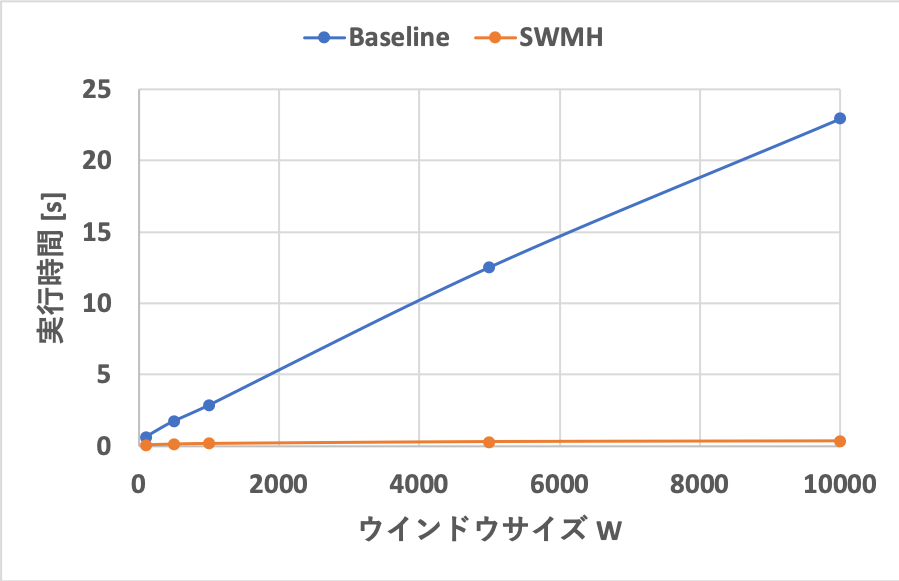
\includegraphics[width=8cm]{SW_connect.png}
      \caption{connect dataset}
    \label{fig:jikken1_3}
      \end{minipage}
         %---- 図はここまで ----------------------
    \end{tabular}
  \end{figure*}
  
  

      \begin{figure*}[h]
  \centering
  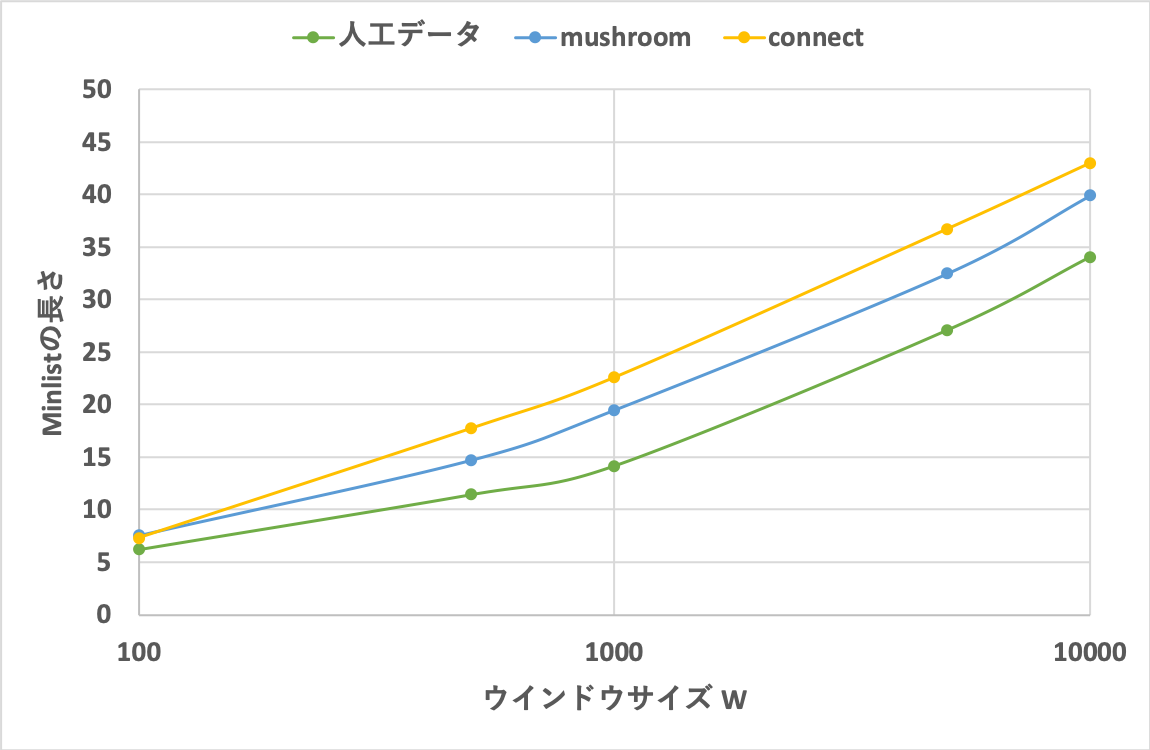
\includegraphics[width=14cm]{jikken1_SW.png}
    \caption{Wに対するMinlistの長さ}
    \label{fig:jikken1_ML}
\end{figure*}


実験 2):偏りパラメータ$\alpha$を変えて実験

偏り $\alpha = [0,1]$の幅で$0.1$ごとに変えて,SWMHの実行時間とMinlistの長さを計測した.%(図 \ref{fig:jikken2}).

人工データ, connect, mushroomいずれのデータセットにおいても,SWMHがBaselineより早かった(図\ref{fig:jikken2}).Baselineでは,偏りが大きくなるにつれて実行時間が短くなることに対して,SWMHでは実行時間が長くなっていく.これは,偏りが大きいほど要素の出現に偏りができ,ハッシュ値計算時の割り当て値表へのアクセスが局所的になり,キャッシュ効率が改善したためBaselineは実行時間が短くなったと考えられる.
しかし,SWMHでは,偏りが大きくなるごとに同じ要素が多く出やすくなる影響から4.2.3のアルゴリズムによりMinlistスキャンの際に,ヒストグラムや割り当て表を深く参照する回数が増える一方で,Minlistの長さに大きな影響を与えないため実行時間が長くなっていると考えられる.
%しかし,SWMHでは,偏りが大きいほどMinlist内で違うラベルを持つ要素より,同じラベルを持つ要素にMinlist内の要素は消され,更新されることが増える(図\ref{fig:same_another}).これは,同じラベルによりMinlistを更新する際に,ウインドウに含まれているラベルの要素数を保持しているヒストグラムにアクセスすることが増えるために,実行時間が遅くなっていくことが考えられる.
表\ref{tab:jikken2},図\ref{fig:same_another}より,Minlistの長さは,$\alpha$が増えるごと途中までは,増加するが,途中から減少する.これは,$\alpha$が大きくなるにつれて,Minlist内の要素が違うラベルによって消される減少量より,同じラベルに消される増加量が大きくなっていくことにより,起きていると考えられる.

%さらに,$\alpha = [0 ,1]$の幅で0.1ごとに変えて,提案手法の実行時間とMinlistの長さを計測した(表 \ref{tab:jikken2}).

%図 \ref{fig:jikken2} より,Baselineでは,偏りが上がるごとに実行時間が短くなることに対して,MHI4では実行時間が長くなっていく.これは,傾きが大きいほど,要素の出現に偏りができ,Baselineでは割り当て表へのアクセスが数箇所に集中し,時間が短くなったことが考えられる.しかし,提案手法では,傾きが大きいほどMinlist内で違うラベルを持つ要素より,同じラベルを持つ要素にMinlist内の要素は消され,更新されることが増える.これは,同じラベルによりMinlistを更新する際に,ウインドウに含まれているラベルの要素数を保持しているヒストグラムにアクセスすることが増えるために,実行時間が遅くなっていくことが考えられる.

 \begin{figure*}[h]
  \centering
  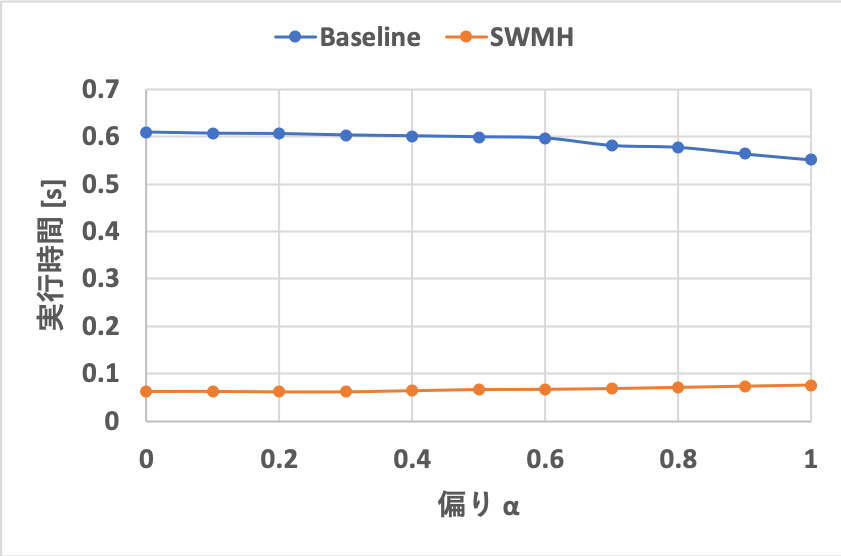
\includegraphics[width=14cm]{katamuki.png}
    \caption{傾き$\alpha$を変えた実行時間}
    \label{fig:jikken2}
\end{figure*}
  
  \begin{figure*}[h]
  \centering
  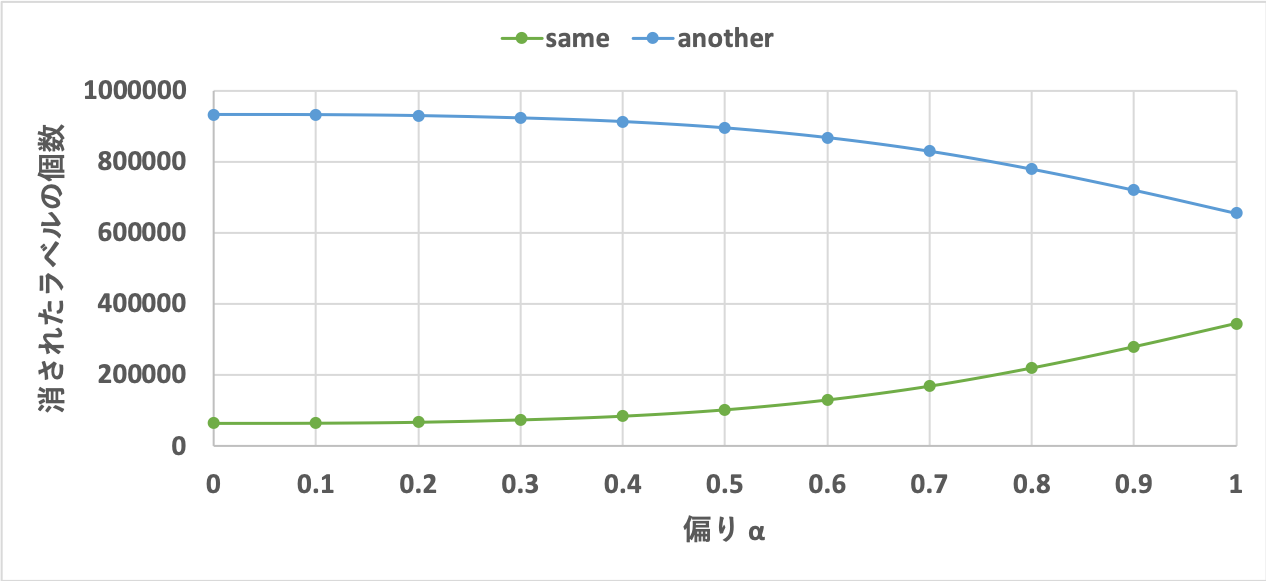
\includegraphics[width=14cm]{same_another.png}
    \caption{Minlistの消去されたラベルの種類}
    \label{fig:same_another}
\end{figure*}


\begin{table}[h]
 \caption{傾きと実行時間,Minlistの長さとの関係}
  \label{tab:jikken2}
 \centering
 \scalebox{0.8}{
  \begin{tabular}{|c| |r|r|r|r|r|r|r|r|r|r|r|}
 
   \hline
    傾き& 0 & 0.1 & 0.2  & 0.3 & 0.4 & 0.5 & 0.6 & 0.7 & 0.8 & 0.9 & 1\\
  
   \hline \hline
   実行時間[s] & 0.06311 & 0.0631 & 0.06227 & 0.06238 & 0.06454 & 0.0668 & 0.6732 & 0.06885 & 0.0711 & 0.07347 & 0.07577 \\
   \hline
   Minlistの長さ & 6.44605 & 6.46051 & 6.47262 & 6.52681 & 6.59502 & 6.66685 & 6.75032 & 6.81968 & 6.62904 & 6.54369 & 6.29902 \\
   \hline
 
  \end{tabular}
  }
\end{table}


実験 3):ラベル種類数$|\phi|$の変更

要素の種類数 $| \phi | = 10,50,100,500$と変えて,提案手法の実行速度と最小値候補リストMinlistの長さを計測した.
図\ref{fig:jikken3}より,Baselineでは,$|\phi|$が増加すると実行時間が増加する.この理由は,ラベルの種類数が多いほど,割り当て値表の広範囲にアクセスし,アクセスが局所的でなくなった結果,キャッシュ効率が限定的にないためと思われる.
一方で,SWMHでは,ラベルの種類数が増えるほど,Minlist更新の際に,同じラベルを持つ要素同士の削除が減少し,実行時間が減っていくと考えられる.


  \begin{figure*}[h]
  \centering
  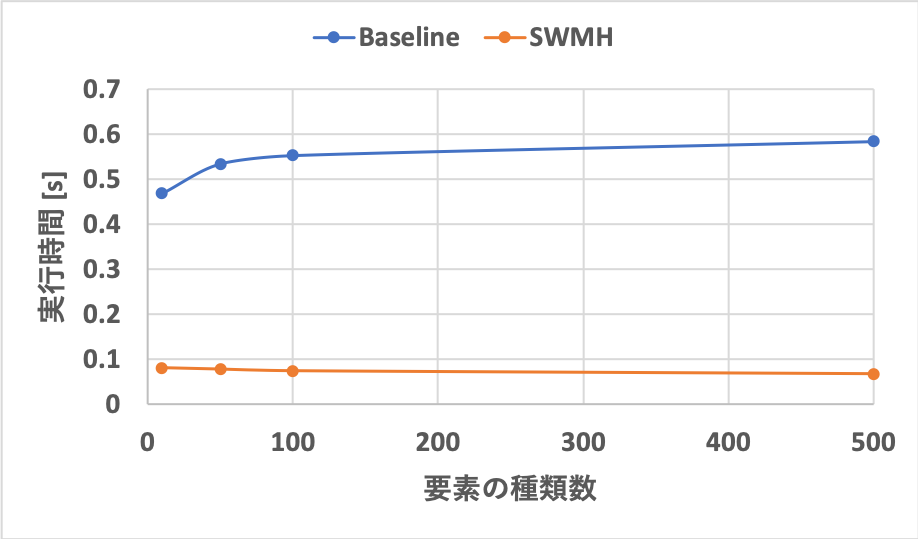
\includegraphics[width=14cm]{jikken3.png}
    \caption{ラベルの種類数$|\phi|$を変えた実行時間}
    \label{fig:jikken3}
\end{figure*}

実験4): ヒストグラム参照上限固定実験

SWMHのアルゴリズムでは,Minlistをスキャンする際に,スキャンされる要素$e'$よりウインドウ内で後ろにある$l(e_{t+1})$の個数に応じた$l(e_{t+1})$の割り当て値を使用し,将来必要ない要素の削除を行なっているが,ヒストグラムを参照する個数の上限を固定してMinlistをスキャンする実験を行う.例えば,上限2の場合,$e'$の後ろに$l(e_{t+1})$が5個あったとしても,$\pi(l(e_{t+1})_{5})$ではなく,$\pi(l(e_{t+1})_{2})$と比べて,$e'$を削除するか判定する.


参照するヒストグラムの個数を固定し,ラベルの種類数 $| \phi | = 10,30,100$と変えて,実行時間を計測した.
図\ref{fig:fix}より,$|\phi| = 10,30$の時は,ヒストグラム参照上限2で実行時間が一番短くなり,$|\phi| = 100$の時は,上限1の実行時間が一番短くなった.ヒストグラムを多く参照しても,Minlistの長さへ与える影響は少なくなり(図\ref{fig:fix_ML}),逆に何回も割り当て表やヒストグラムを参照することに時間をかけていると考えられる.

 \begin{figure*}[h]
  \centering
  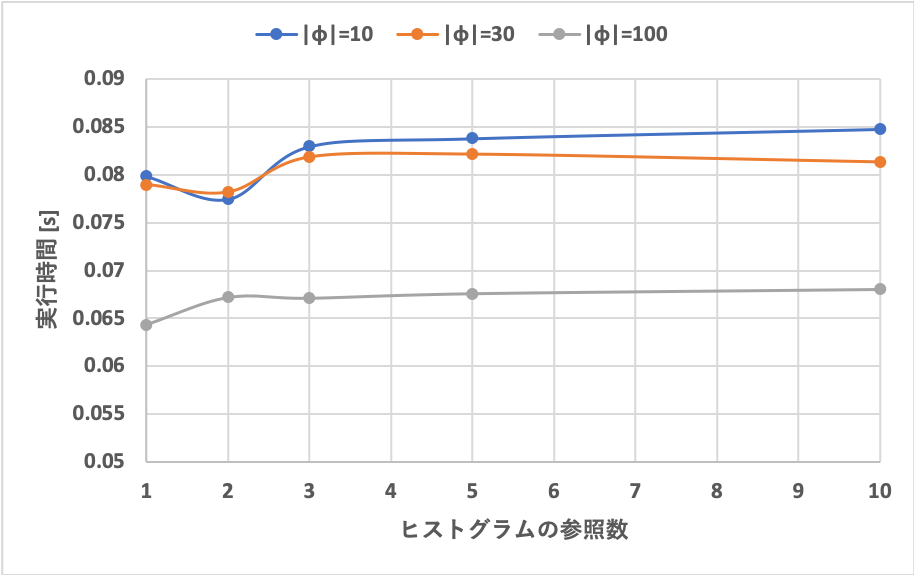
\includegraphics[width=14cm]{jikken_fix.png}
    \caption{ヒストグラムの参照数を変えた実行時間}
    \label{fig:fix}
\end{figure*}

 \begin{figure*}[h]
  \centering
  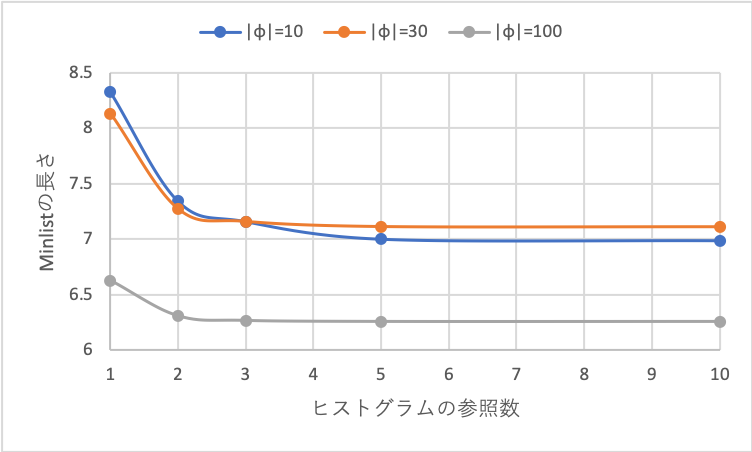
\includegraphics[width=14cm]{jikken_fix_ML.png}
    \caption{ヒストグラムの参照数を変えたMinlist}
    \label{fig:fix_ML}
\end{figure*}

\section{バッチSWMHの実験評価}
本実験では,人工データとconnect,mushroomの3つのデータセットを使用した.まず,人工データを使った評価主数を説明する.人工データのパラメータは到着レート$c = 5$,$\alpha = 1$, $|\phi|=100$,$W = 100$という組み合わせをデフォルトパラメータとし,実験を行なった.次に,実データを使った評価主数を説明する.実データのパラメータは,$c = 5$,$W=100$をデフォルトパラメータとし,実験を行なった.実験において,実験のばらつきを減らすためにハッシュ関数を10個生成し,バッチSWMHの合計を実行時間として,実験を行なった.

%実験 5): バッチSWMHの実行時間の計測
人工データ, connect, mushroomいずれのデータセットにおいても,SWMHを$c$回適応する方法より,バッチSWMHの方が約2倍早かった(表\ref{tab:jikken4_1} ).図\ref{tab:jikken4_2}より,Minlistの長さはバッチSWMHの方が長くなった.SWMHでは,c回スキャンするため,$c$個の要素のアルファベットを使用するが,バッチSWMHでは$c$個の要素のうち2個の要素のアルファベットのみを使用し,削除するためにMinlistが長くなっていると考えられる.しかし,入ってきた要素すべてとMinlist内の要素を比較して候補とならない要素を消していくのではなく,入ってきた要素の中から最小値となり得る要素を厳選し,その要素を用いて削除していくことによりMinlistを更新する回数を減らし,実行時間を短縮することができたと考えられる.


%SWMHとバッチSWMHを比較して実験し,バッチ SWMHの実行時間と最小値候補リストMinlistの長さを計測した.実験では,バッチSWMHのウインドウに一回に入ってくる要素数:5として実験を行なった(表\ref{tab:jikken4_1} ,表\ref{tab:jikken4_2}).
%実験結果より,SWMHより実行時間が短くなっていることがわかる.Minlistを更新する際に,入ってきた要素すべてとMinlist内の要素を比較して候補とならない要素を消していくのではなく,入ってきた要素の中から最小値となり得る要素を厳選し,その要素を用いて削除していくことによりMinlistを更新する回数を減らし,実行時間を短縮することができた.

\begin{table}[h]   
          \caption{バッチSWMHの実行時間}
        \label{tab:jikken4_1}
 \centering
  \begin{tabular}{|c| |c|c|c|}
   \hline
    データセット & 人工 & connect & mushroom\\
   \hline \hline
   SWMH & 0.0742 & 0.0743 & 0.073 \\
   \hline
   バッチSWMH & 0.042 & 0.0365 & 0.037 \\
   \hline
     \end{tabular}
  \end{table}
 
      
\begin{table}[h]
        \caption{バッチSWMHのMinlistの長さ}
          \label{tab:jikken4_2}
           \centering
  \begin{tabular}{|c| |c|c|c|}
   \hline
    データセット & 人工 & connect & mushroom\\
   \hline \hline
   SWMH & 6.2883 & 6.2082 & 6.296\\
   \hline
   バッチSWMH & 6.5501 & 7.5545 & 7.4214 \\
   \hline
    \end{tabular}
  \end{table}







\chapter{まとめ}
 本研究ではデータストリームに対する類似検索の高速化を念頭に,データストリームに対するハッシュ値の更新アルゴリズムを取り扱った.とくにスライディングウィンドウを動的に変化する多重集合と見なして,スライディングウィンドウに対するMin-Hashのハッシュ値更新アルゴリズムSWMHを提案した.SWMHはスライディングウィンドウで集合を取り扱ったDatarらの手法を多重集合に拡張したものであり,スライディングウインドウモデルで多重集合を取り扱える初の手法である.
  SWMHの特筆すべき点は,動的多重集合に対してMin-hashを計算する場合,1つの要素への割り当て値が多重度に影響されて動的に変化するという難点に対応したことである.さらに要素への割り当て値をハッシュ値が変化しない範囲で修正することにより,SWMHが管理する必要がある要素数を削減させて,実行時間を短縮した.
さらに,SWMHを拡張し,一度に複数個の要素がスライディングウインドウに到着するモデルに対応したMin-hash計算手法であるバッチSWMHを提案した.バッチSWMHでは,要素1つ1つに対してMinlistを更新するのではなく,ウインドウに入ってきた要素群の中で,最小の割り当て値を保持する要素と最大多重度のラベルを保持する要素の2つに絞り,Minlistへアクセスする回数を減らすことで実行時間の短縮を狙った.
 人工datasetと実データセットを用いてMin-hash計算時間を測る実験を行い,提案手法を評価した.まず,SWMHは,毎時刻Min-hashのハッシュ値を再計算するベースラインより,高速にハッシュ値を算出できることを示せた.さらに,バッチSWMHは,複数個の要素がウインドウを出入りする場合にSWMHより短い時間でMin-hashを高速計算できることを示した.
 最後に,提案手法SWMHでは,データを保持するためにヒストグラムを多用しているため,多くのメモリを消費している.従って,今後の研究課題としては,メモリ使用量の削減のために近似ヒストグラムを用いてハッシュ値を計算する手法の実現が望まれる.


\vspace{2em}

\begin{thebibliography}{99}
  \bibitem{Datar}
 Mayur Datar and S Muthukrishnan "Estimating Rarity and Similarity over Data Stream Window" AT\&T Research, Florham Park NJ, USA.

  \bibitem{Xu2016}
  X, Xu,C. Gao, J. Pei, K.Wang, and A. Al-Barakati,"Continuous similarity search for evolving queries," Knowledge and Information Systems, vol.48(3),pp.649-678, September 2016.

\bibitem{HistoSketch}
Yang D, Li B, Rettig L, Cudre-Mauroux P. "HistoSketch : fast similarity  preserving sketching of streaming histograms with concept drift", 2017 IEEE international conference on data mining (ICDM); 2017. p. 545-54.
        
\bibitem{Maxloghash}
Wang P, Qi Y, Zhang Y, Zhai Q, Wang C, Lui J, Guan X. "A Memory-Efficient Sketch Method for Estimating High Similarities in Streaming Sets",  2019.

\bibitem{b-bit}
Ping Li, Arnd Christian Konig, "b-Bit Minwise Hashing", 2010 Nineteenth International World Wide Web Conference (WWW 2010).

\bibitem{dataset2}
Michael M, Rasmus P, Ninh, "Efficient Estimation for High Similarities using Odd Sketches" , In WWW, pages 109-118, 2014.

\bibitem{microbiome}
W PM Rowe, A Paola Carrieri, C Alcon-Giner, S Caim, A Shaw, K Sim, J Kroll, L j.Hall, E O.Pyzer-Knapp, M D.Winn, "Streaming histogram sketching for rapid microbiome analytics" Rowe et al.Microbiome 2019.

\bibitem{POI}
D. Yang, B. Li, and P. Cudre-Mauroux, “Poisketch: Semantic place labeling over user activity streams,” in Proc. of IJCAI, 2016, pp. 2697-2703.

\bibitem{Bury}
M Bury, C Schwiegelshohn, M Sorella, "Efficient Similarity Search in Dynamic Data Streams", 2021.

\bibitem{Minhash}
A Z Broder, M Charikar, A M Frieze, M Mitzenmacher, "Min-Wise Independent Permutations",Journal of Computer and System Sciences Volume 60, Issue 3, June 2000, Pages 630-659.


\bibitem{CWS}
M Manasse, F McSherry, K Talwar, "Consistent weighted sampling", 2010.

\end{thebibliography}


\end{document}